% !TeX spellcheck = en_US
% !TeX encoding = UTF-8
\documentclass[10pt, a4paper]{article}
\usepackage{graphics, graphicx}
\usepackage{fancyvrb, enumerate}
\usepackage{amsmath, amssymb, amscd, amsfonts}
\usepackage{geometry}
\usepackage{multirow}
\usepackage{url}
\usepackage{tikz}
\usepackage{listings, listing}
\usepackage{color}
\usepackage{apacite}

\usetikzlibrary{shapes, arrows, calc, positioning}
\definecolor{codegreen}{rgb}{0, 0.6, 0}
\definecolor{codegray}{rgb}{0.5, 0.5, 0.5}
\definecolor{codepurple}{rgb}{0.58, 0, 0.82}
\definecolor{backcolour}{rgb}{0.95, 0.95, 0.92}
\definecolor{mygreen}{RGB}{28,172,0}
\definecolor{mylilas}{RGB}{170,55,241}

\lstdefinestyle{mystyle}
{
	backgroundcolor=\color{backcolour},   
	commentstyle=\color{codegreen},
	keywordstyle=\color{magenta},
	numberstyle=\tiny\color{codegray},
	stringstyle=\color{codepurple},
	basicstyle=\footnotesize,
	breakatwhitespace=false,         
	breaklines=true,                 
	captionpos=b,
	keepspaces=true,                 
	numbers=left,                    
	numbersep=5pt,                  
	showspaces=false,                
	showstringspaces=false,
	showtabs=false,                  
	tabsize=2,
	frame=single
}
\lstset{style=mystyle}
\tikzstyle{decision} = [diamond, draw, fill=blue!20, text width=4.5em, text badly centered, node distance=3cm, inner sep=0pt]
\tikzstyle{block} = [rectangle, draw, fill=blue!20, text width=5em, text centered, rounded corners, minimum height=2em, node distance=2cm]
\tikzstyle{line} = [draw, -latex']
\tikzstyle{cloud} = [draw, ellipse, fill=red!20, node distance=5em, minimum height=2em, node distance=2cm]
\tikzset
{
	-|-/.style=
	{
		to path=
		{
			(\tikztostart) -| ($(\tikztostart)!#1!(\tikztotarget)$) |- (\tikztotarget)
			\tikztonodes
		}
	},
	-|-/.default=0.5,
	|-|/.style=
	{
		to path=
		{
			(\tikztostart) |- ($(\tikztostart)!#1!(\tikztotarget)$) -| (\tikztotarget)
			\tikztonodes
		}
	},
	|-|/.default=0.5,
}

\lstset{language=Matlab,
	breaklines=true,
	morekeywords={matlab2tikz},
	keywordstyle=\color{blue},
	morekeywords=[2]{1}, keywordstyle=[2]{\color{black}},
	identifierstyle=\color{black},
	stringstyle=\color{mylilas},
	commentstyle=\color{mygreen},
	showstringspaces=false,
	numbers=left,
	numberstyle={\tiny \color{black}},
	numbersep=9pt,
	emph=[1]{for,end,break},emphstyle=[1]\color{red},  
}

\geometry
{
	top = 20mm,
	bottom = 20mm,
	left = 20mm,
	right = 20mm
}

\title{FID Data Reconstruction and $T_1$, $T_2$, $T_2^{*}$ Fitting}
\author{20161206 JaewoongLee}
\date{\today}

\begin{document}
    \maketitle
	\newpage
	
	\tableofcontents
	\listoftables
	\listoffigures
	\newpage
	
	\section{Theory}
		\subsection{Magnetic Resonance Imaging}
			Magnetic Resonance Imaging (MRI) is a medical imaging technique used in radiology to form pictures of the anatomy and the physiological process of the body. The basis of MRI techniques is the measurement of radio-frequency radiation resulting from transition induced between nuclear spin states of tissue hydrogen protons in the presence of a strong external magnetic field. \cite{ref:MRI1}
			
			The two parameters that are often used to characterize the behavior of an MRI signal and which can be used as a basis for generating MRI contrast are the spin-lattice (T1) and spin-spin (T2) relaxation times. \cite{ref:MRI1}
			
		\subsection{Free Induction Decay}
			Free induction decay (FID) is the observable MRI signal generated by non-equilibrium nuclear spin magnetization precessing about the magnetic field. \cite{ref:MRI2}
			
			\begin{figure}[htbp]
				\centering
				$\begin{array}{cc}
					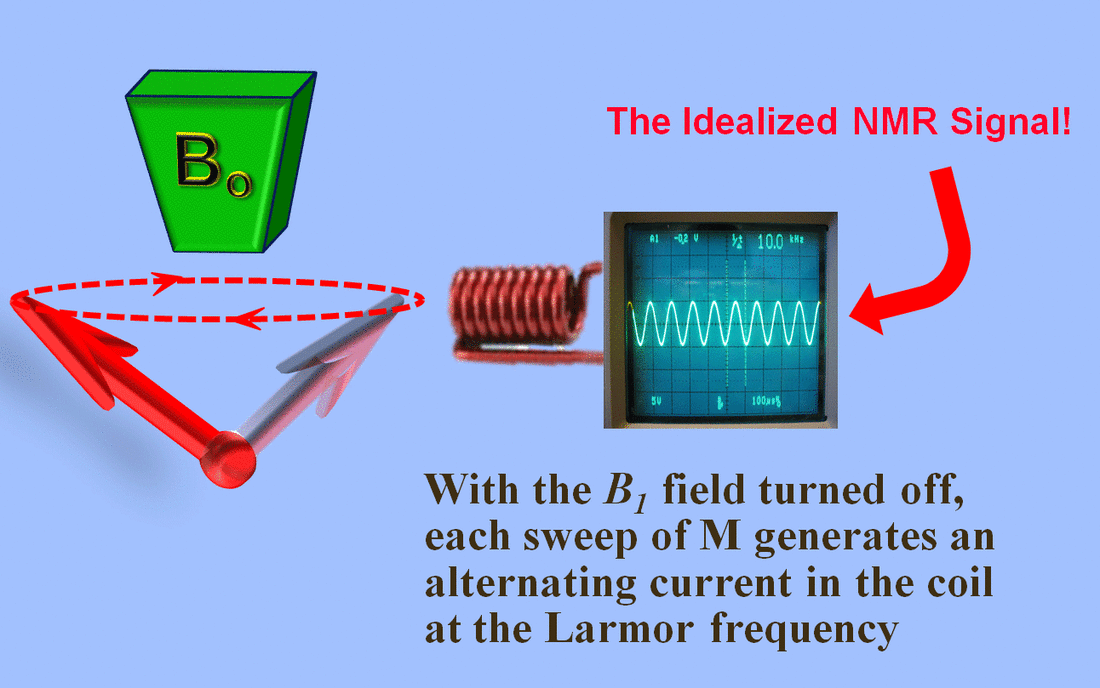
\includegraphics[width=0.3 \linewidth]{figures/FID1.png}
					&
					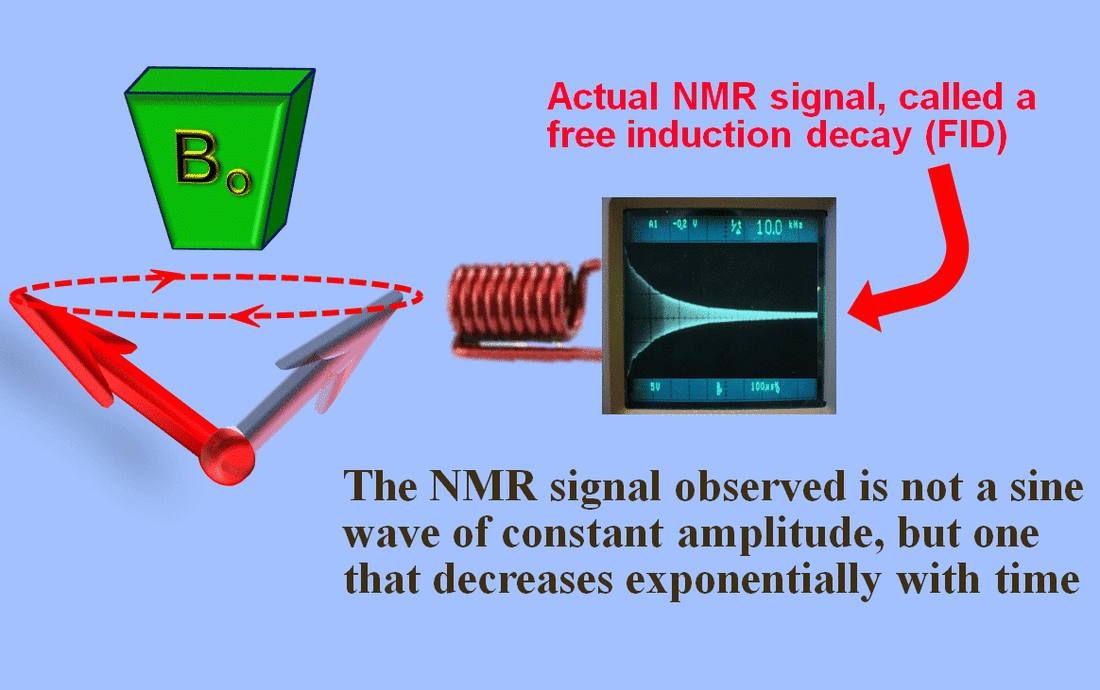
\includegraphics[width=0.3 \linewidth]{figures/FID2.png}
					\\
					
					\mbox{(a) Idealized Signal}
					&
					\mbox{(b) Actual Signal}
				\end{array}$
				\caption{Ideal and Actual Signal \protect \cite{ref:MRI2}}
				\label{fig:fid}
			\end{figure}
		
		\subsection{Fourier Transform}
			A Fourier Transform (TF) is a mathematical transform which decomposes a function in to its constituent frequencies. Also, there are two main algorithm in TF: Discrete Fourier Transform (DFT) and Fast Fourier Transform (FFT). The FFT algorithm derives its efficiency by replacing the computation of one large DFT with that of several smaller DFTs. \cite{ref:FFT1}
			
		\subsection{Brain Development}
			Over and over again, the basic stages and mechanisms of mammalian brain development has been made in our understanding. In \textit{Homo sapience}, the brain development is a protracted process that begins in the third gestational week, and it continues for an extended period post-natally. \cite{ref:brain1} Some papers addressed MRI studies of structural and functional changes in the developing human brain and their relation to changes in cognitive processes over the first decades of human life. \cite{ref:brain2}
			
			\subsubsection{Substantia nigra}
				The substantia nigra (SN) is an anatomically heterogeneous nucleus with regional alternation in striatal projections and distribution of histo-chemical markers. \cite{ref:nigra1} It is well-known than degenerative diseases of the SN indicate regional selectivity, and the SN has around 50 neuronal groups. 
				
				Moreover, dopamin contributes to the processing of signals in the SN. \cite{ref:nigra3} It has long been known that dopamine is released to regulate not only the neurotransmitter from the SN, but also the activity of the dopaminergic neurons. \cite{ref:nigra2} Also, the dopaminergic neurons have been developed in the SN. \cite{ref:nigra4} Hence, the substantia nigra has an important role in dopamine distribution. 
			
			\subsubsection{Corpus callosum}
				The corpus callosum (CC) is a wide and thick nerve tract, consisting of a flat bundle of commissural fibers, beneath the cerebra cortex in the brain. The CC, as the main inter-hemispheric fiber tract, plays an major role in inter-hemispheric integration and communication. \cite{ref:cc1} 
				
				The size of CC differs upon their diseases, occupations, and genders. In schizophrenic patients, the CC would be smaller than normal. \cite{ref:cc2} The CC also would be decreased in autistic, even they are non-mentally retarded. \cite{ref:cc3} The CC would increase between 30 professional musicians and matched controls. \cite{ref:cc1} Some papers suggest a sex difference in the CC. \cite{ref:cc4}
				
				The growth of the CC was checked from the fourth fetal month to maturity, even in the adulthood. \cite{ref:cc5, ref:cc6} The CC has a major role in inter-hemispheric functional connectivity in the motor and auditory cortices; the agenesis of CC will diminish the functional connectivity. \cite{ref:cc7}
				
			\subsection{Development in Rats and Humans}
				Obviously, rats and human are different races. Therefore, there are no exact one-to-one connection between development of rats and humans. There are something, such as tail, which rats have but humans do not; and vice versa. Even though, some papers made approximate one-to-one correspond between development of rats and humans. \cite{ref:dev1, ref:dev2}
				
				\begin{figure}[htbp]
					\centering
					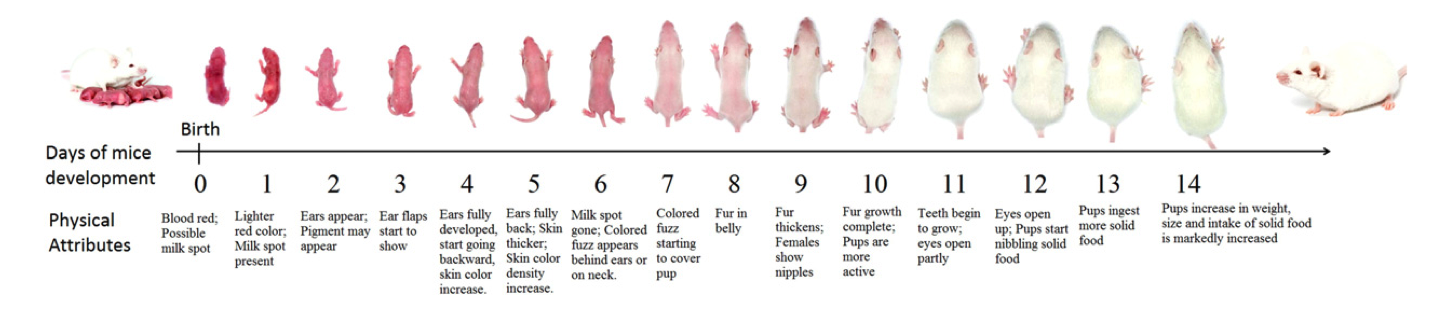
\includegraphics[width=0.8 \linewidth]{figures/development.png}
					\caption{The approximate age of mice can be determined by their physical attributes during the first 2 weeks of life \protect \cite{ref:dev1}}
				\end{figure}
			
				Thus, the relation between rats and human aging is as the table \ref{tb:dev}.
				
				\begin{table}[htbp]
					\centering
					\caption{The rat's age in months and its relationship in years with human being in social maturity phase \protect \cite{ref:dev2}}
					\label{tb:dev}
					\begin{tabular}{cc}
						Rat's age in months & Human's age in years \\ \hline
						6 month & 18 years \\
						12 month & 30 years \\
						18 month & 45 years \\
						24 month & 60 years \\
						30 month & 75 years \\
						36 month & 90 years \\
						42 month & 105 years \\
						45 month & 113 years \\
						48 month & 120 years \\
					\end{tabular}
				\end{table}
			
				Hence, the following relationship will be used:
				\begin{itemize}
					\item 6 week in Rat = 4.5 years in Human
					\item 4 month in Rat = 12 years in Human
					\item 20 month in Rat = 50 years in Human
				\end{itemize}
	
	\section{Method}
		In this section, the example code will be displayed. However, there are many repetition parts in the program; in this case, only the first part will be shown. Also, there are three types of data:
		\begin{enumerate}
			\item RARE-VTR: Rapid Acquisition with Relaxation Enhancement with Variable repetition time TR
			\item MSME: Multi-Slice Multi-Echo
			\item MGE: Multi-Gradient Echo
		\end{enumerate}
		Three types of data will be used in $T_1$, $T_2$, and $T_2^*$ analysis, respectively.
	
		\subsection{Initializing}
			In this step, the parameters which will be used in entire program will be set, and the raw data are loaded. 
			
			\lstinputlisting[language=matlab, firstline=5, lastline=25]{../FID_recon_and_fitting.m}
	
		\subsection{FID Data Reconstruction}
			In this step, the k-space is re-constructed from the raw data by the Inverse Fourier Transform algorithm. Also, the MRI images are derived from the k-space. 
		
			\lstinputlisting[language=matlab, firstline=67, lastline=96]{../FID_recon_and_fitting.m}
		
		\subsection{$T_1$, $T_2$, $T_2^*$ Fitting}
			In this step, $T_1$, $T_2$, $T_2^*$ fitting is performed with the average of signal. The average of signal is calculated by the equation \ref{eq:average}.
			
			\begin{equation}
				\rm{Average} = \frac{\Sigma \ Signal}{\rm{Number \ of \ Signal}}
				\label{eq:average}
			\end{equation}
		
			\lstinputlisting[language=matlab, firstline=270, lastline=289]{../FID_recon_and_fitting.m}
		
		\subsection{$T_1$, $T_2$, $T_2^*$ Mapping}
			$T_1$, $T_2$, $T_2^*$ Mapping is executed on all of the voxels in the images. 
		
			\lstinputlisting[language=matlab, firstline=448, lastline=471]{../FID_recon_and_fitting.m}
		
		\subsection{Analysis $T_1$, $T_2$, $T_2^*$  by Age}
			In previous sections, the data from not only 6 week but also 4 and 20 month are analyzed. Therefore, no more procedures for analyzing 4 and 20 month data. 
	
	\section{Results}
		\subsection{FID Data Reconstruction}
			\subsubsection{RARE-VTR FID Image}
				In the figure \ref{fig:vtr_6week_image}, there are 10 MRI images from RARE-VTR FID data. The repetition time (TR) is increasing while in the images in figure \ref{fig:vtr_6week_image}. By comparing the image \ref{fig:vtr_6week_image}-(1) and the image \ref{fig:vtr_6week_image}-(10), increasing TR is enhancing the $T_1$ weighted image.
				\begin{figure}[htbp]
					\centering
					$\begin{array}{ccc}
						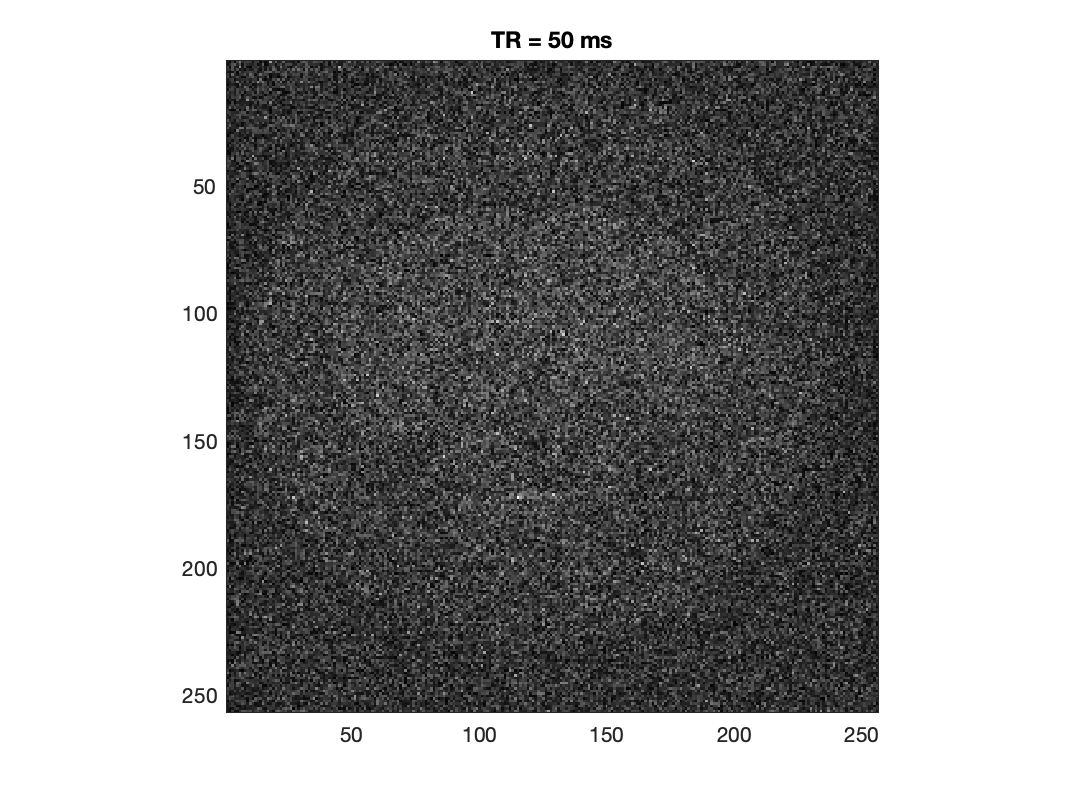
\includegraphics[width=0.3 \linewidth]{figures/VTR_6week/vtr_6week_1.png}
						&
						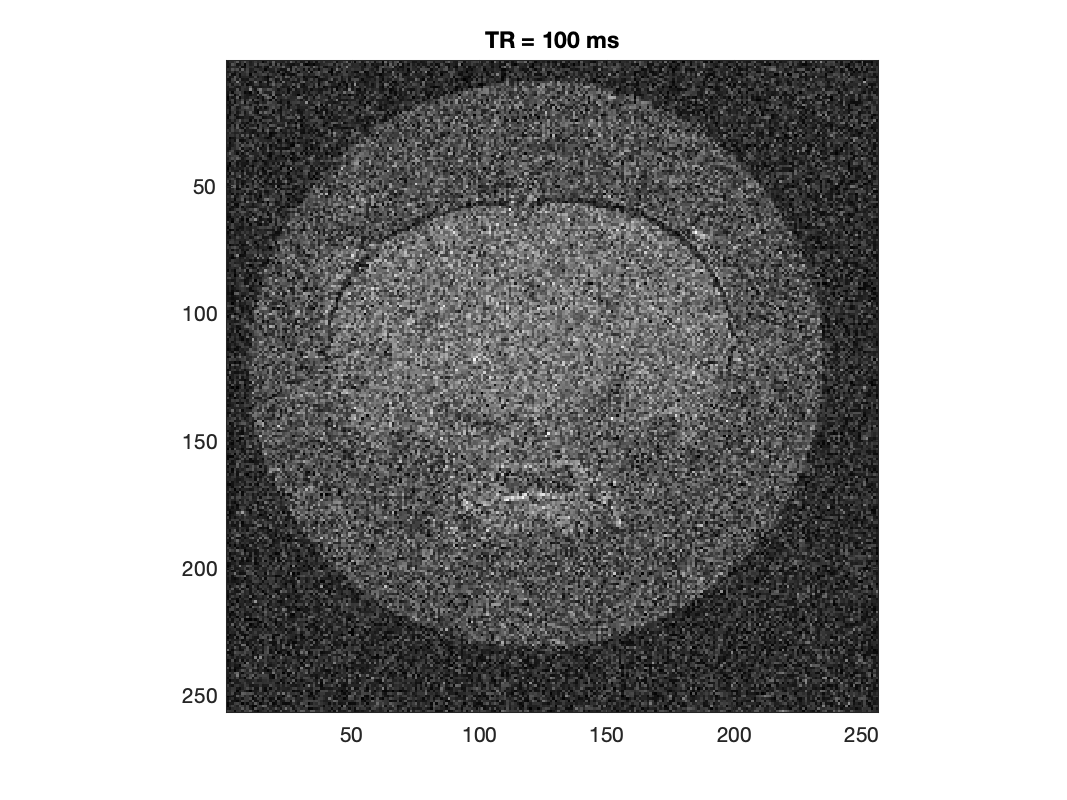
\includegraphics[width=0.3 \linewidth]{figures/VTR_6week/vtr_6week_2.png}
						&
						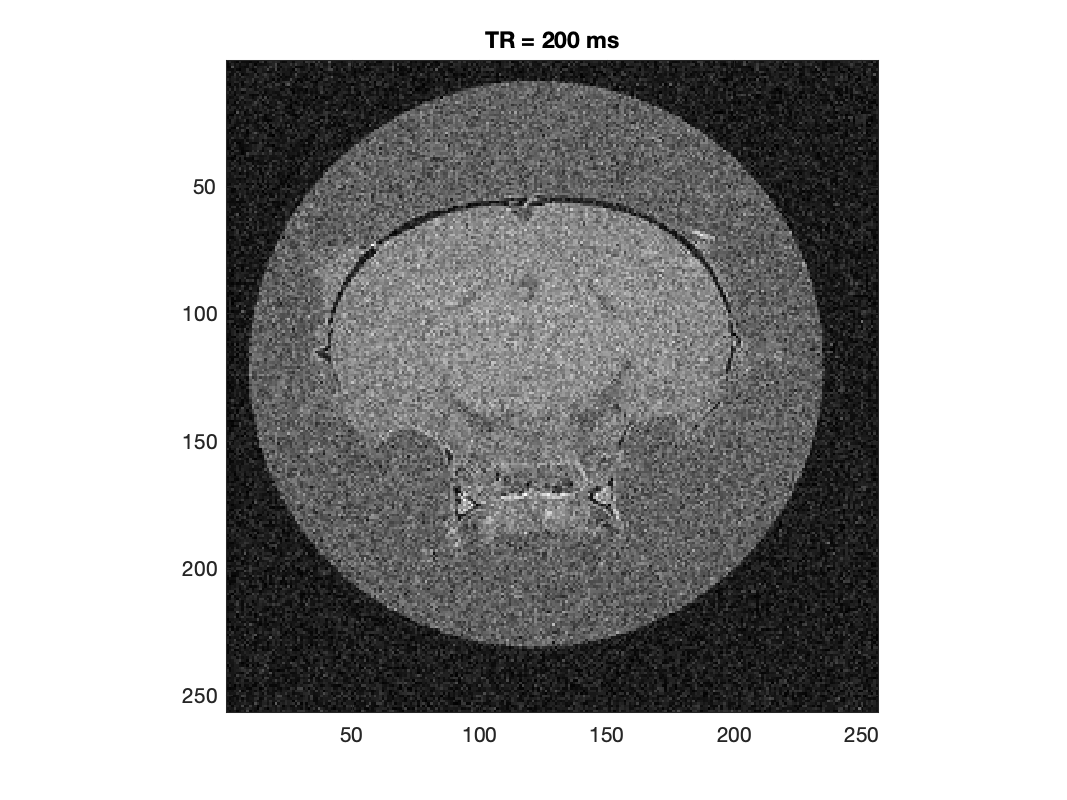
\includegraphics[width=0.3 \linewidth]{figures/VTR_6week/vtr_6week_3.png}
						\\
						\mbox{(1)} & \mbox{(2)} & \mbox{(3)} \\
						
						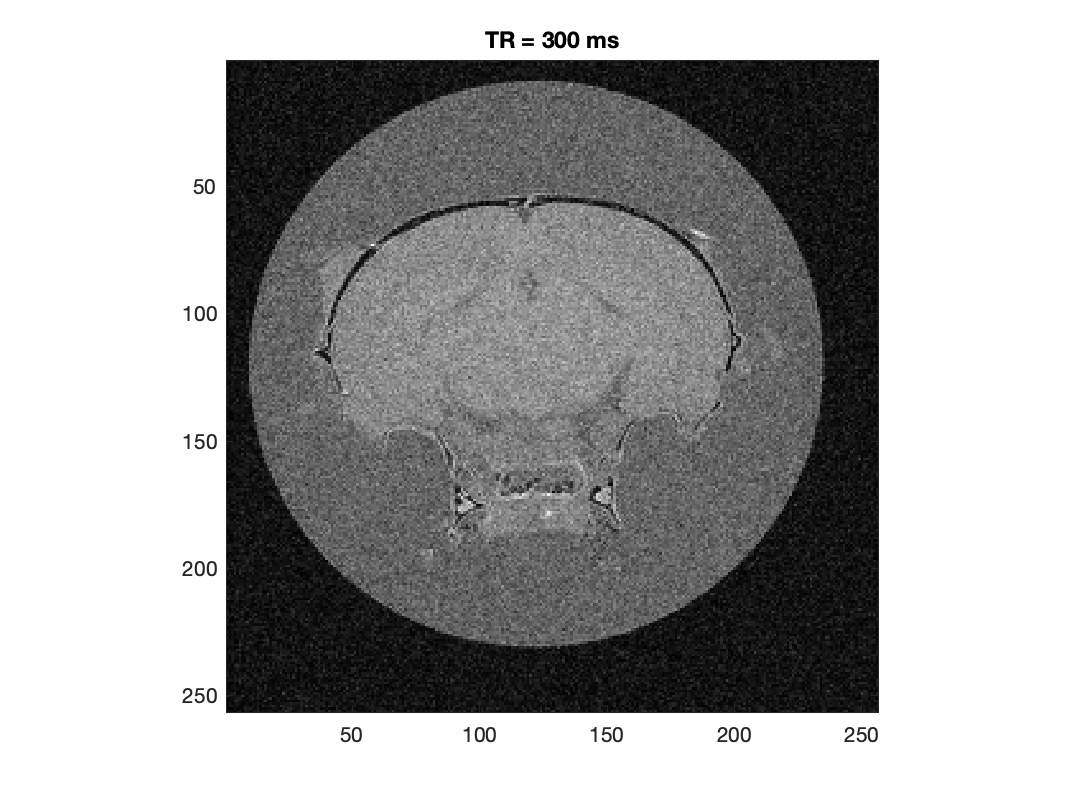
\includegraphics[width=0.3 \linewidth]{figures/VTR_6week/vtr_6week_4.png}
						&
						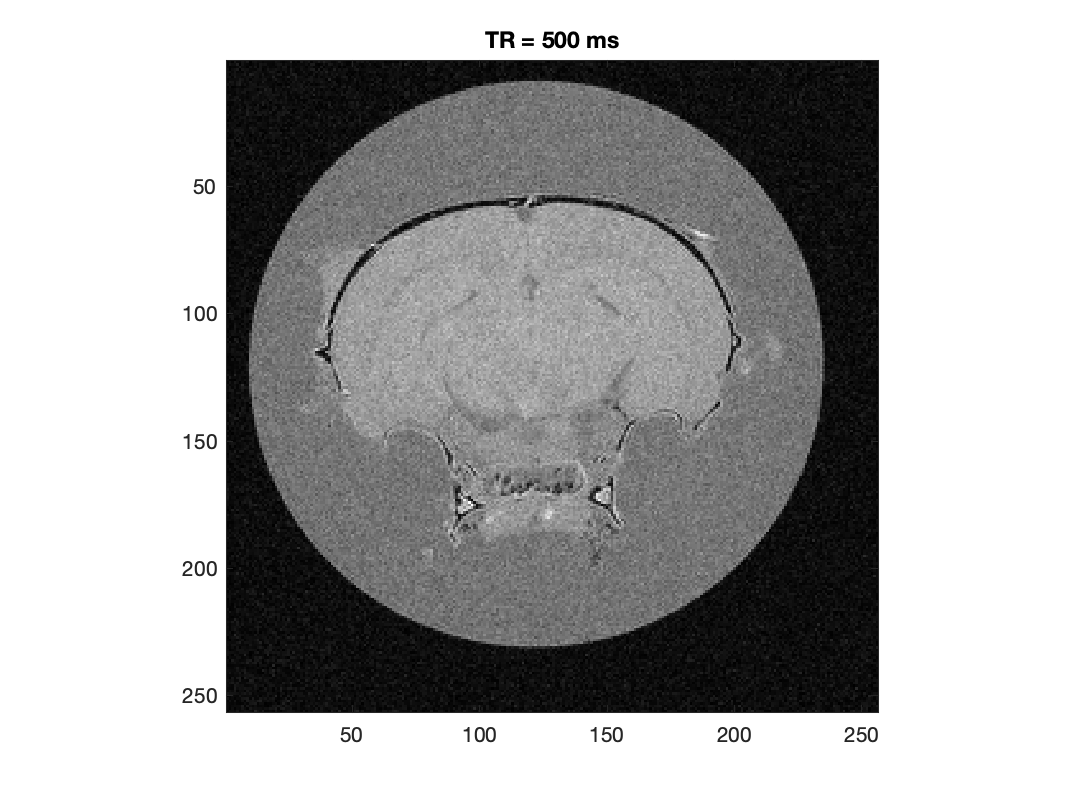
\includegraphics[width=0.3 \linewidth]{figures/VTR_6week/vtr_6week_5.png}
						&
						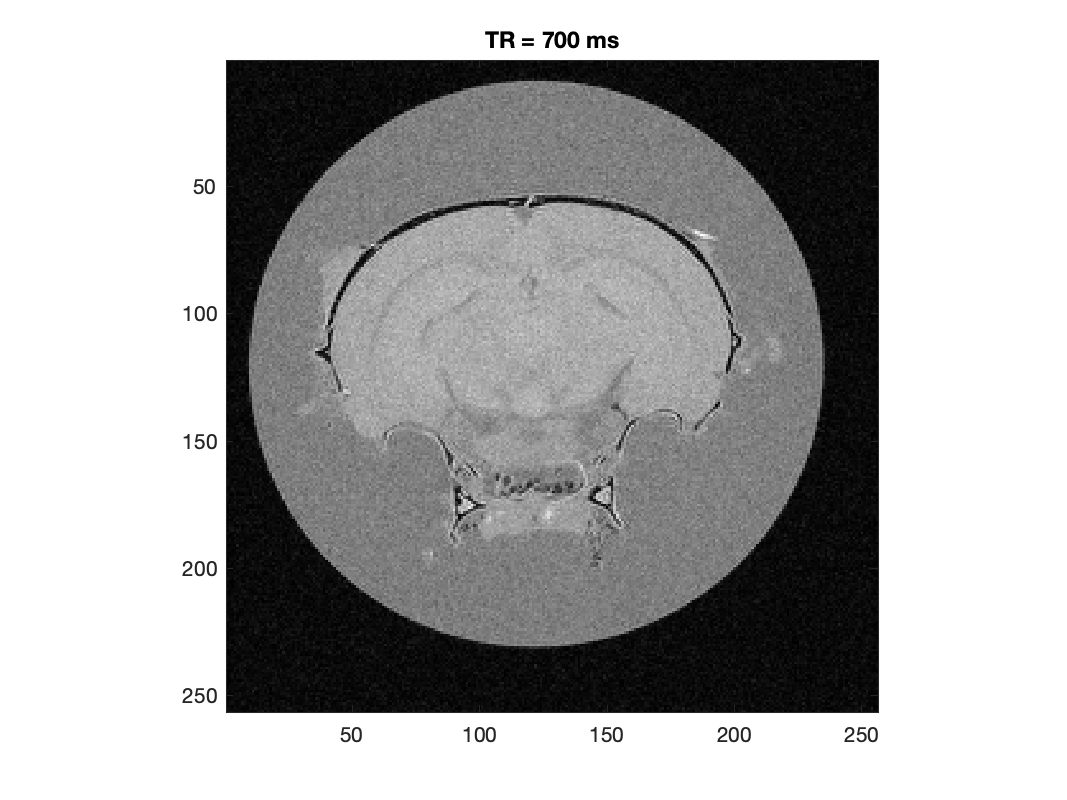
\includegraphics[width=0.3 \linewidth]{figures/VTR_6week/vtr_6week_6.png}
						\\
						\mbox{(4)} & \mbox{(5)} & \mbox{(6)} \\
						
						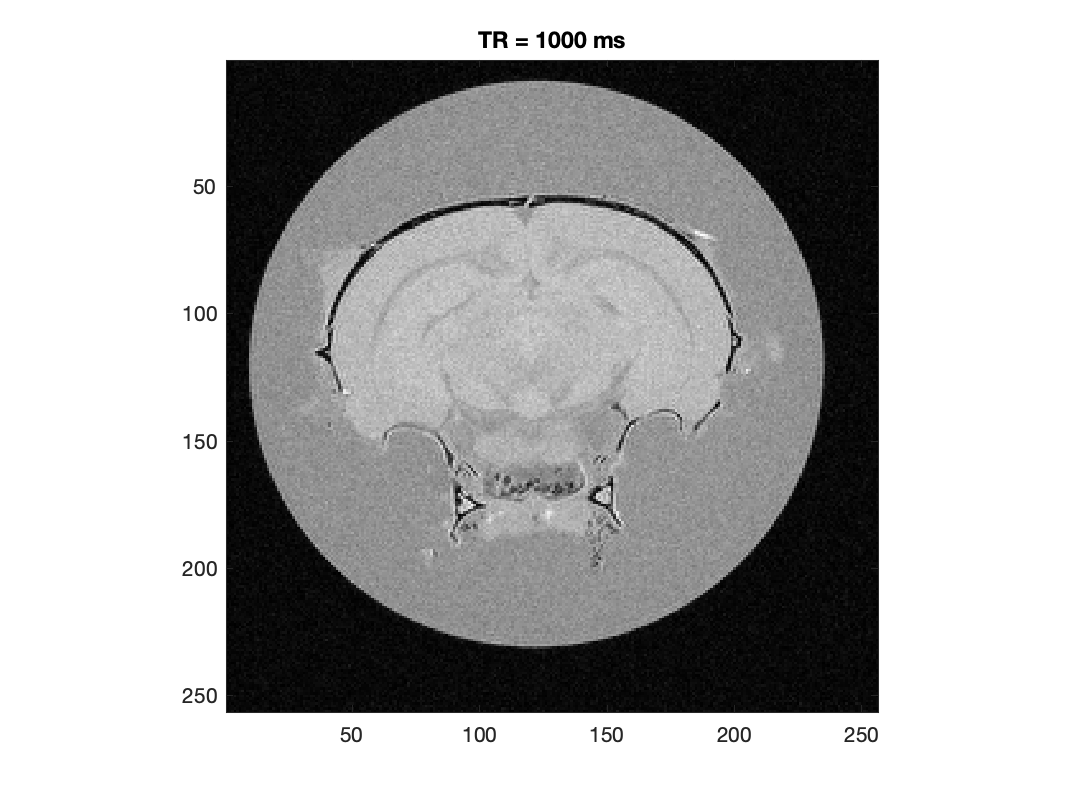
\includegraphics[width=0.3 \linewidth]{figures/VTR_6week/vtr_6week_7.png}
						&
						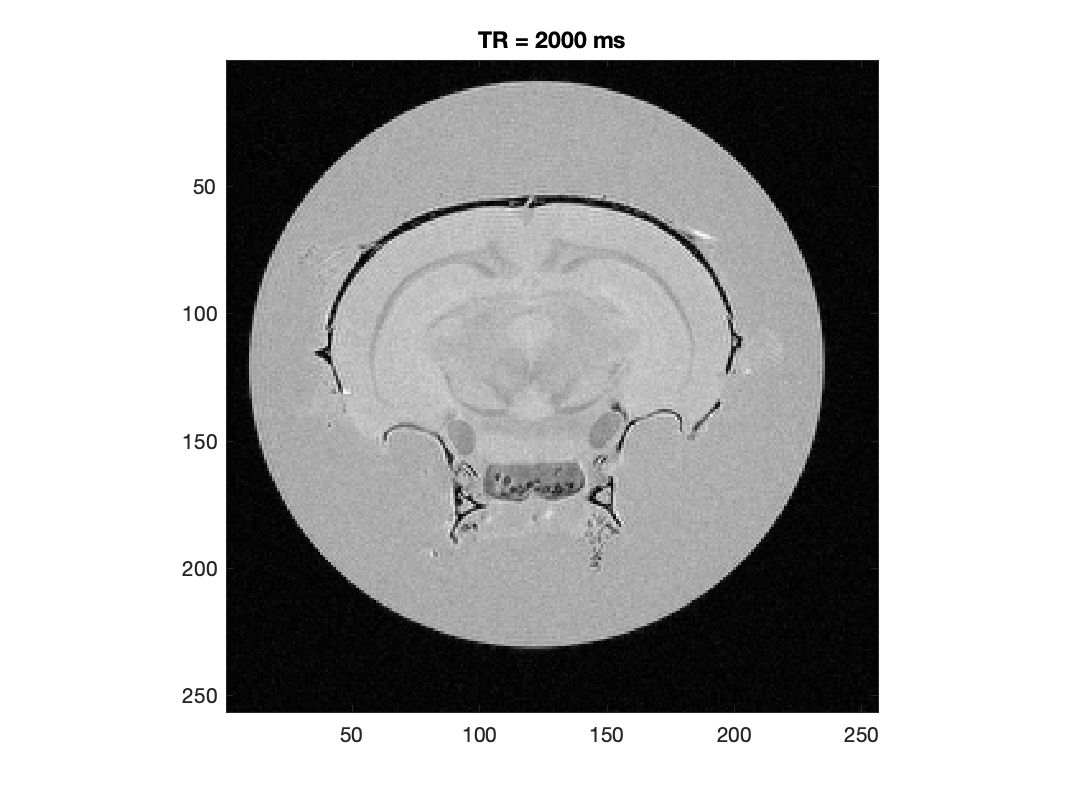
\includegraphics[width=0.3 \linewidth]{figures/VTR_6week/vtr_6week_8.png}
						&
						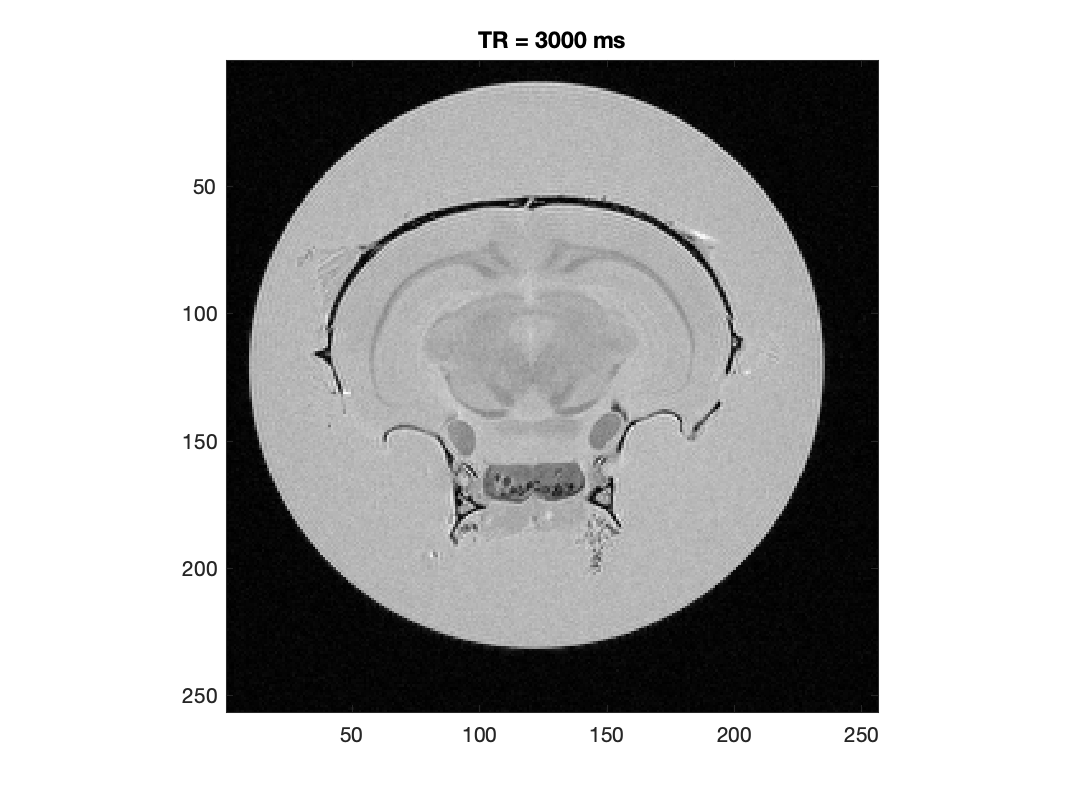
\includegraphics[width=0.3 \linewidth]{figures/VTR_6week/vtr_6week_9.png}
						\\
						\mbox{(7)} & \mbox{(8)} & \mbox{(9)} \\
						
						&
						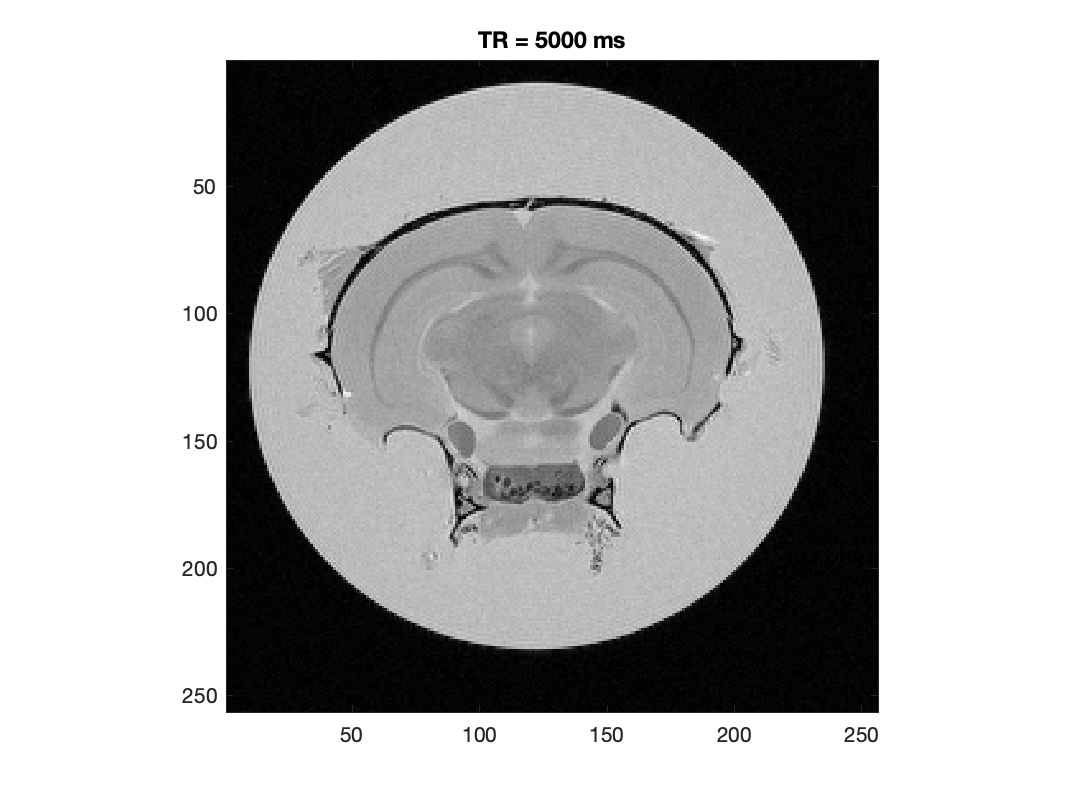
\includegraphics[width=0.3 \linewidth]{figures/VTR_6week/vtr_6week_10.png}
						&
						\\
						& \mbox{(10)} & \\
					\end{array}$
					\caption{RARE-VTR FID Images in 6 Week}
					\label{fig:vtr_6week_image}
				\end{figure}
		
			\subsubsection{MSME FID Image}
				In the figure \ref{fig:msme_6week_image}, there are 48 MRI images from MSME data. The echo time (TE) is increasing on the figure \ref{fig:msme_6week_image}. By comparing the image \ref{fig:msme_6week_image}-(1) and the image \ref{fig:msme_6week_image}-(48), decreasing TR is enhancing the $T_2$ weighted image. 
				\begin{figure}[htbp]
					\centering
					$\begin{array}{cccccc}
						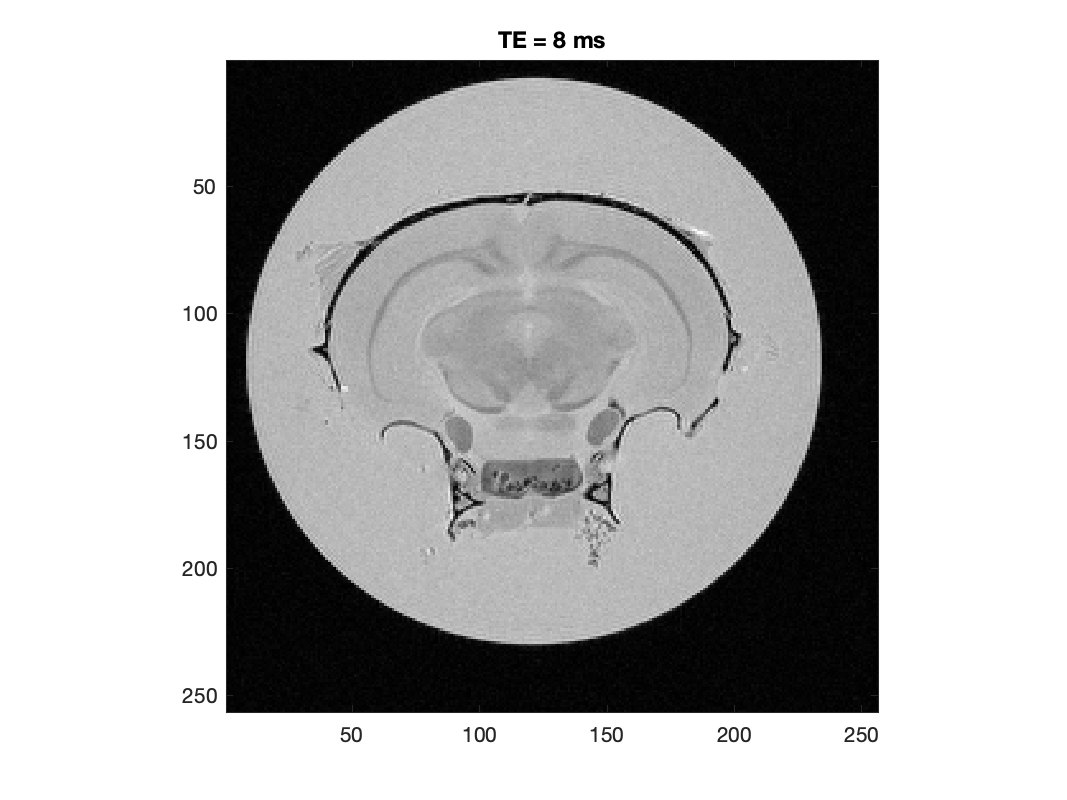
\includegraphics[width=0.15 \linewidth]{figures/MSME_6week/msme_6week_1.png}
						&
						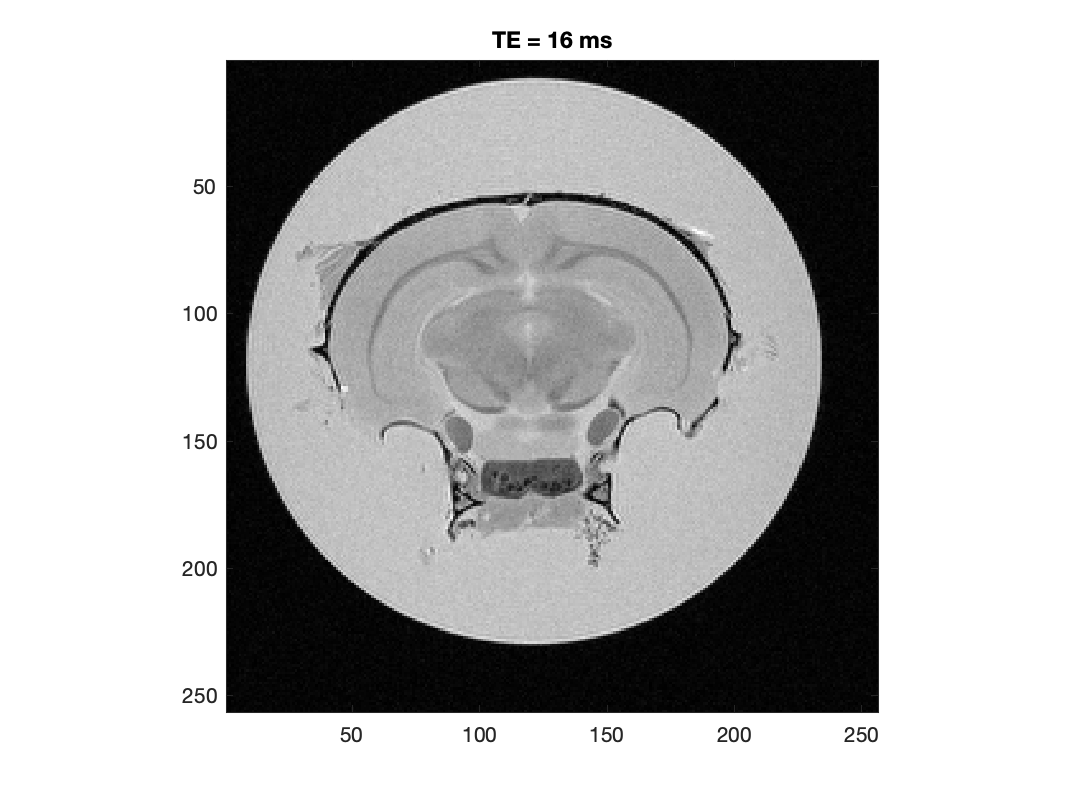
\includegraphics[width=0.15 \linewidth]{figures/MSME_6week/msme_6week_2.png}
						&
						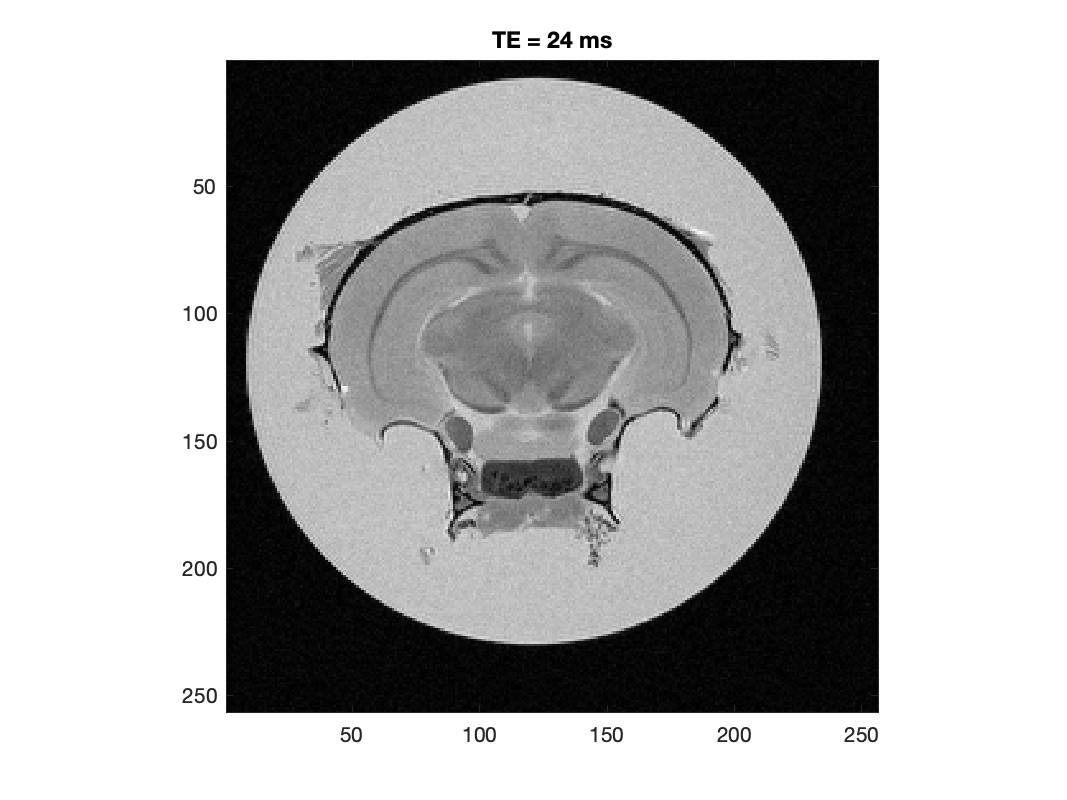
\includegraphics[width=0.15 \linewidth]{figures/MSME_6week/msme_6week_3.png}
						&
						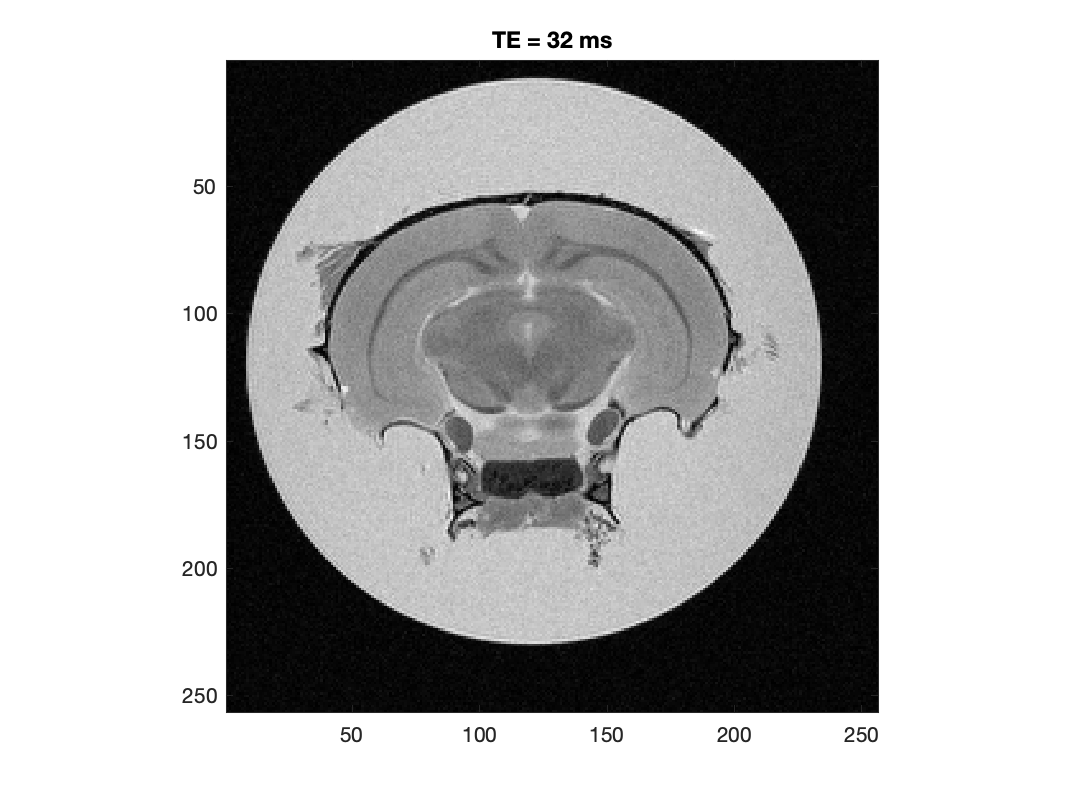
\includegraphics[width=0.15 \linewidth]{figures/MSME_6week/msme_6week_4.png}
						&
						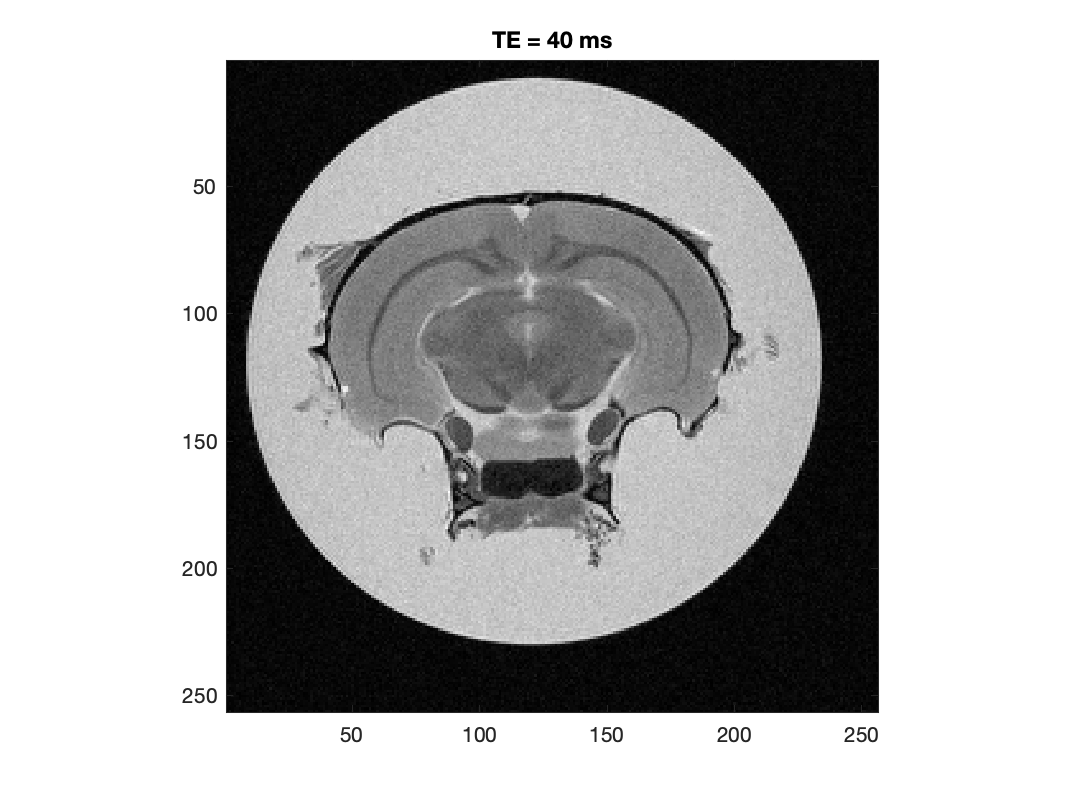
\includegraphics[width=0.15 \linewidth]{figures/MSME_6week/msme_6week_5.png}
						&
						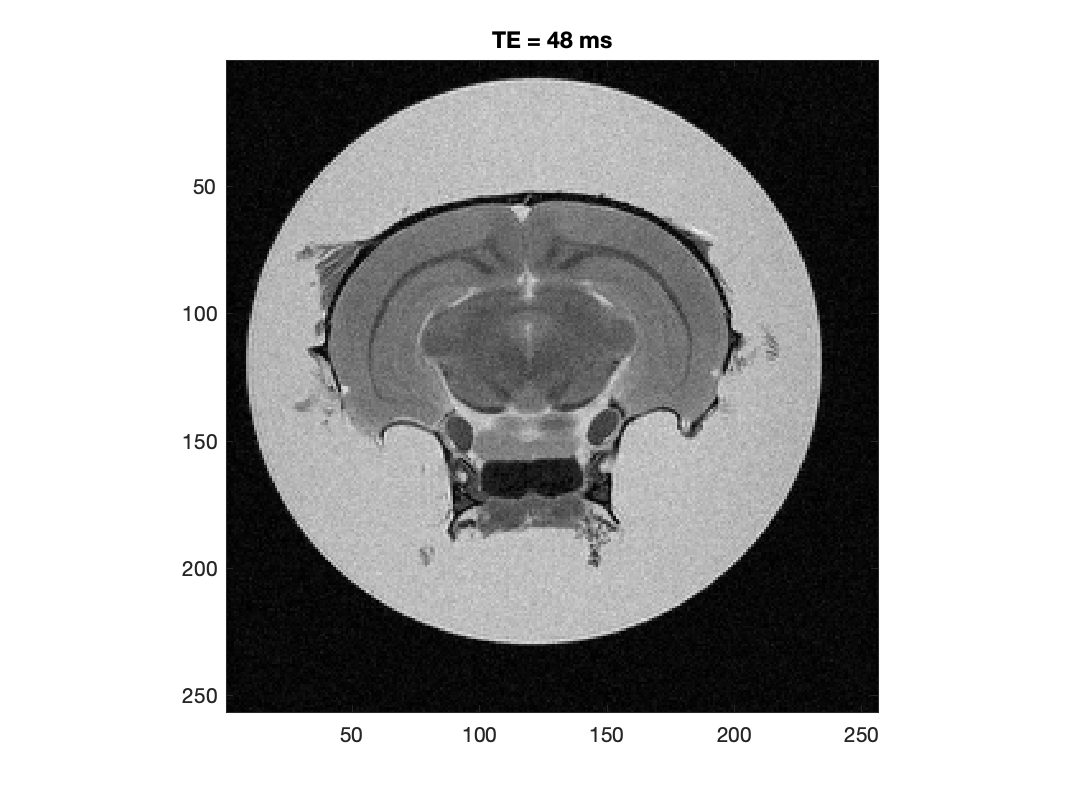
\includegraphics[width=0.15 \linewidth]{figures/MSME_6week/msme_6week_6.png}
						\\
						\mbox{(1)} & \mbox{(2)} & \mbox{(3)} & \mbox{(4)} & \mbox{(5)} & \mbox{(6)} \\
						
						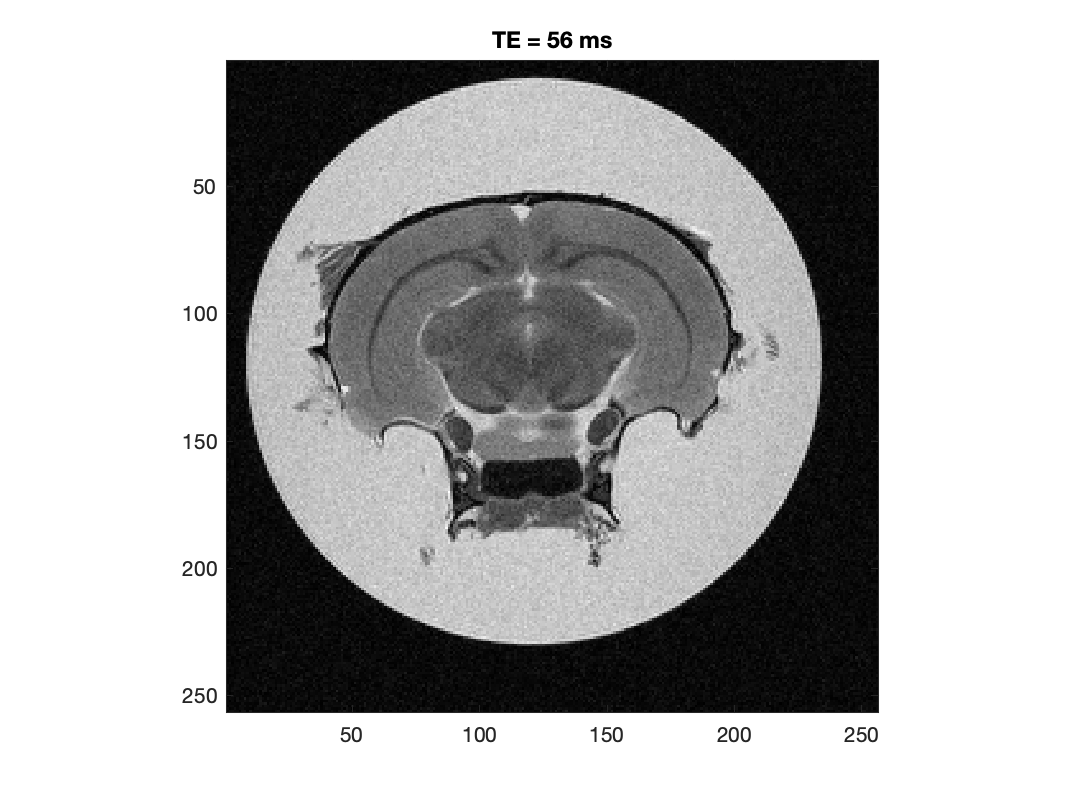
\includegraphics[width=0.15 \linewidth]{figures/MSME_6week/msme_6week_7.png}
						&
						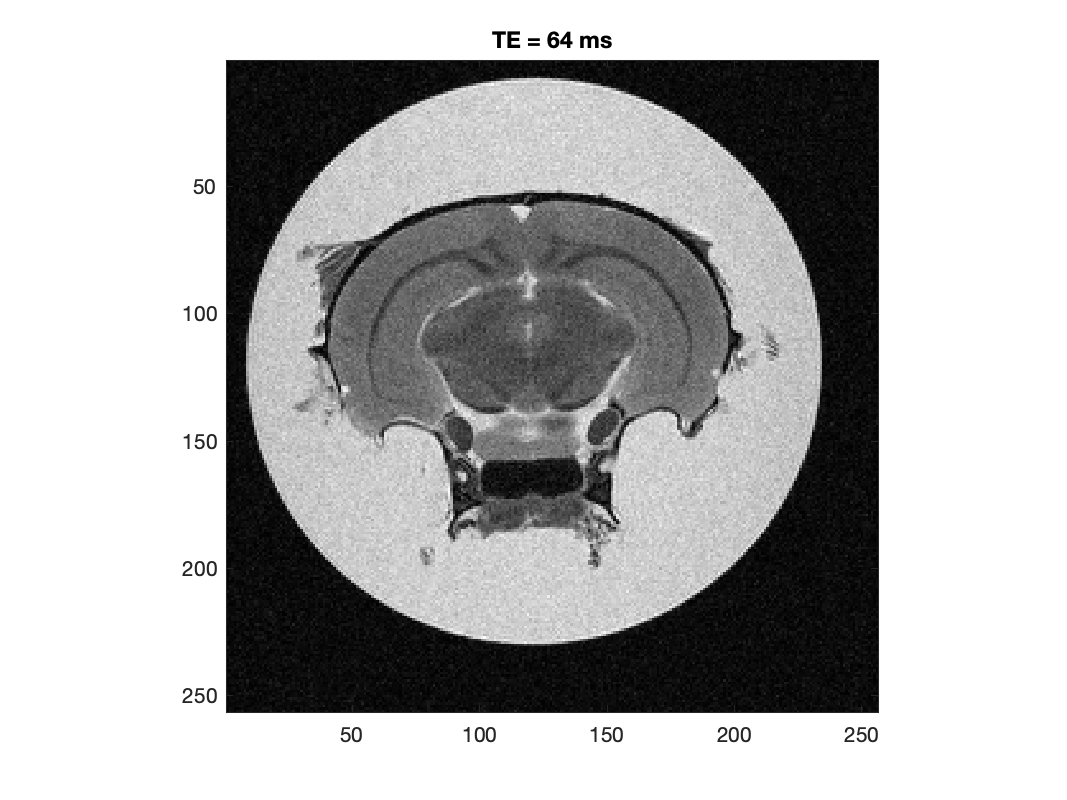
\includegraphics[width=0.15 \linewidth]{figures/MSME_6week/msme_6week_8.png}
						&
						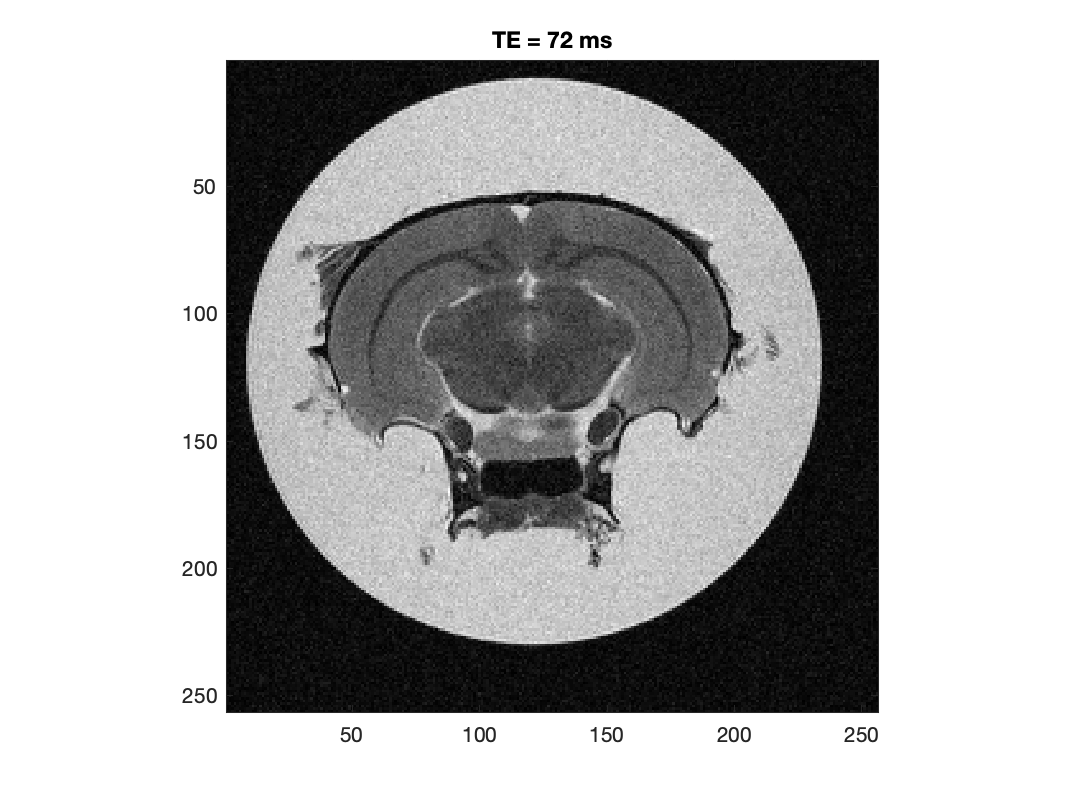
\includegraphics[width=0.15 \linewidth]{figures/MSME_6week/msme_6week_9.png}
						&
						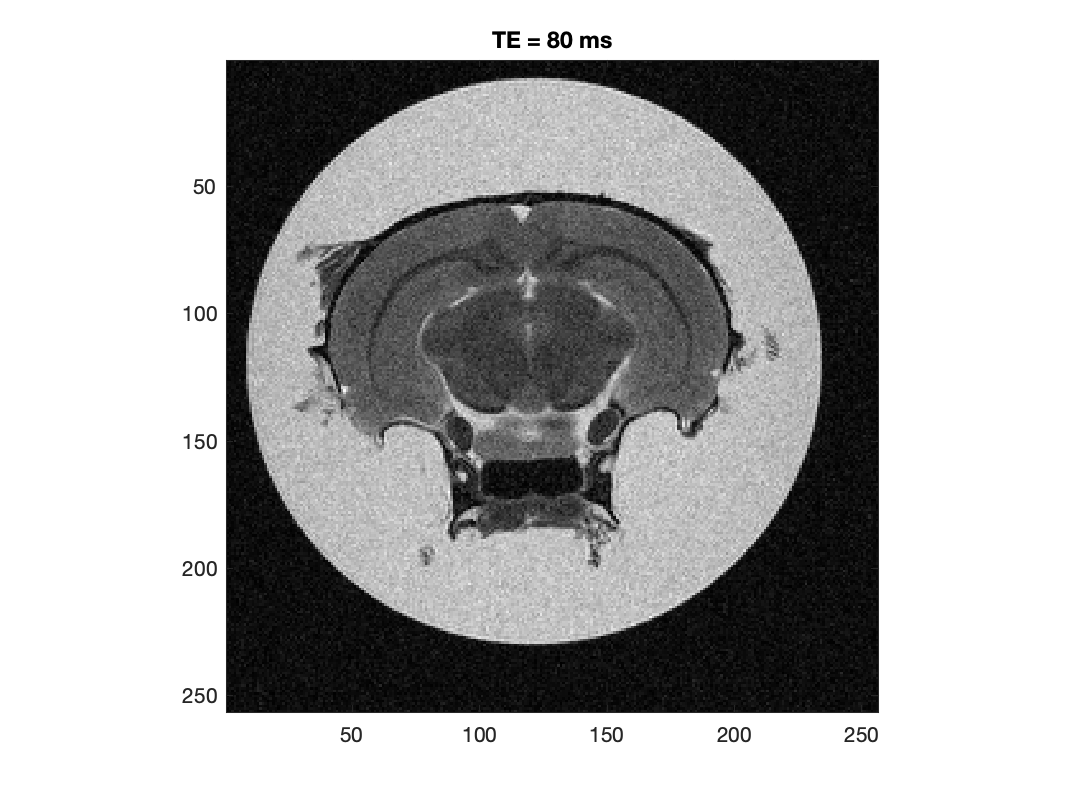
\includegraphics[width=0.15 \linewidth]{figures/MSME_6week/msme_6week_10.png}
						&
						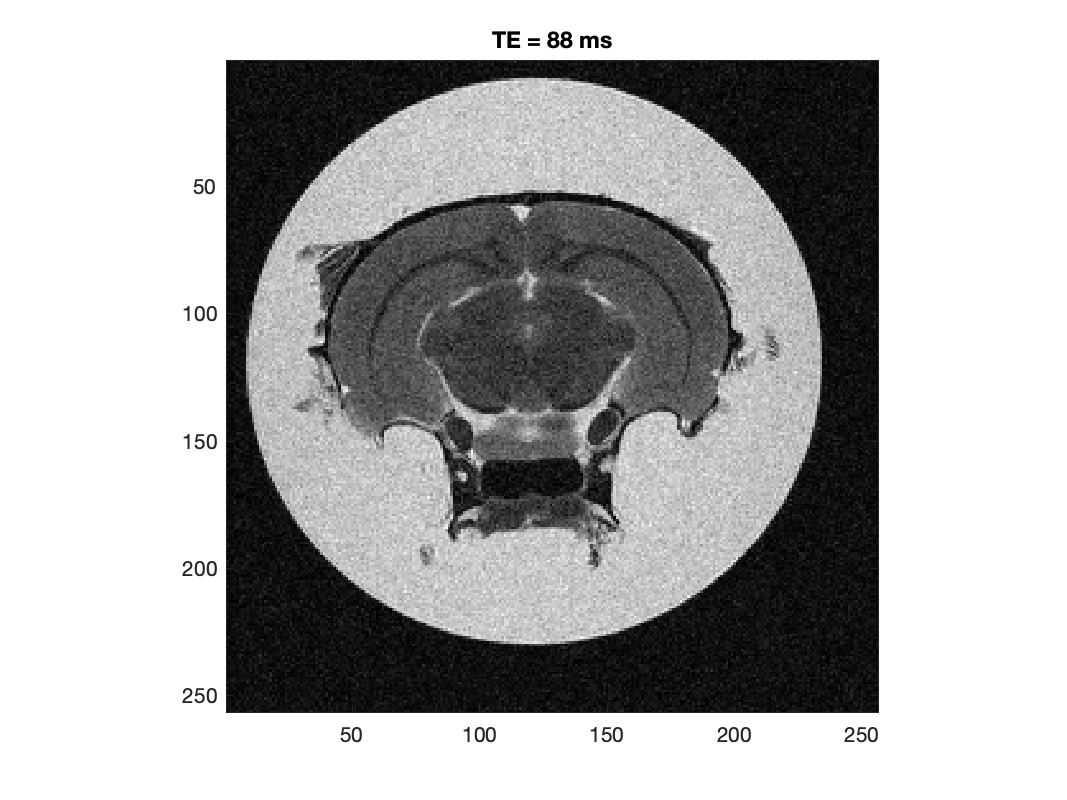
\includegraphics[width=0.15 \linewidth]{figures/MSME_6week/msme_6week_11.png}
						&
						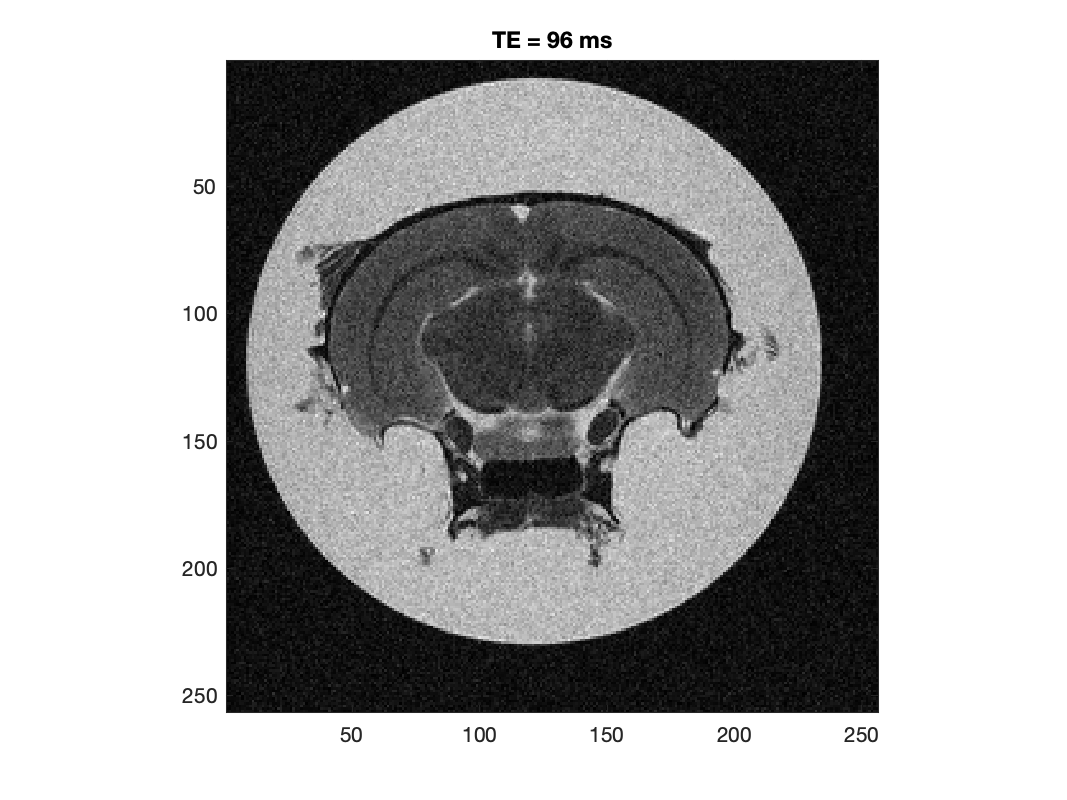
\includegraphics[width=0.15 \linewidth]{figures/MSME_6week/msme_6week_12.png}
						\\
						\mbox{(7)} & \mbox{(8)} & \mbox{(9)} & \mbox{(10)} & \mbox{(11)} & \mbox{(12)} \\
						
						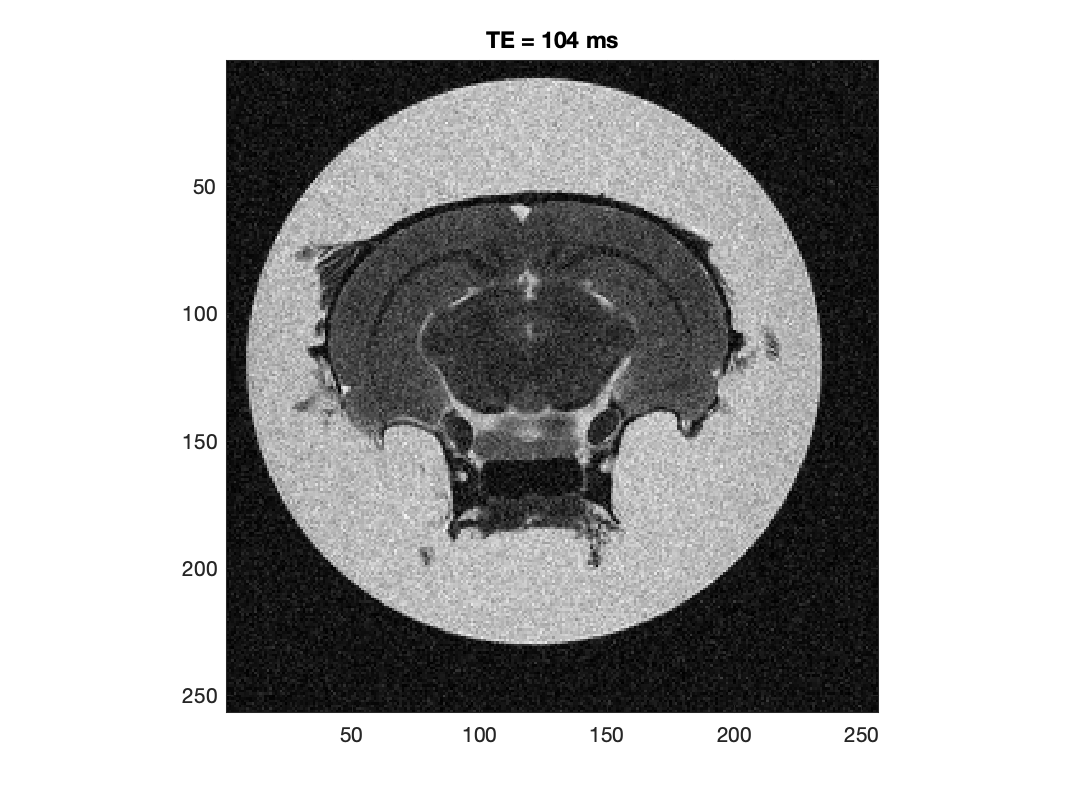
\includegraphics[width=0.15 \linewidth]{figures/MSME_6week/msme_6week_13.png}
						&
						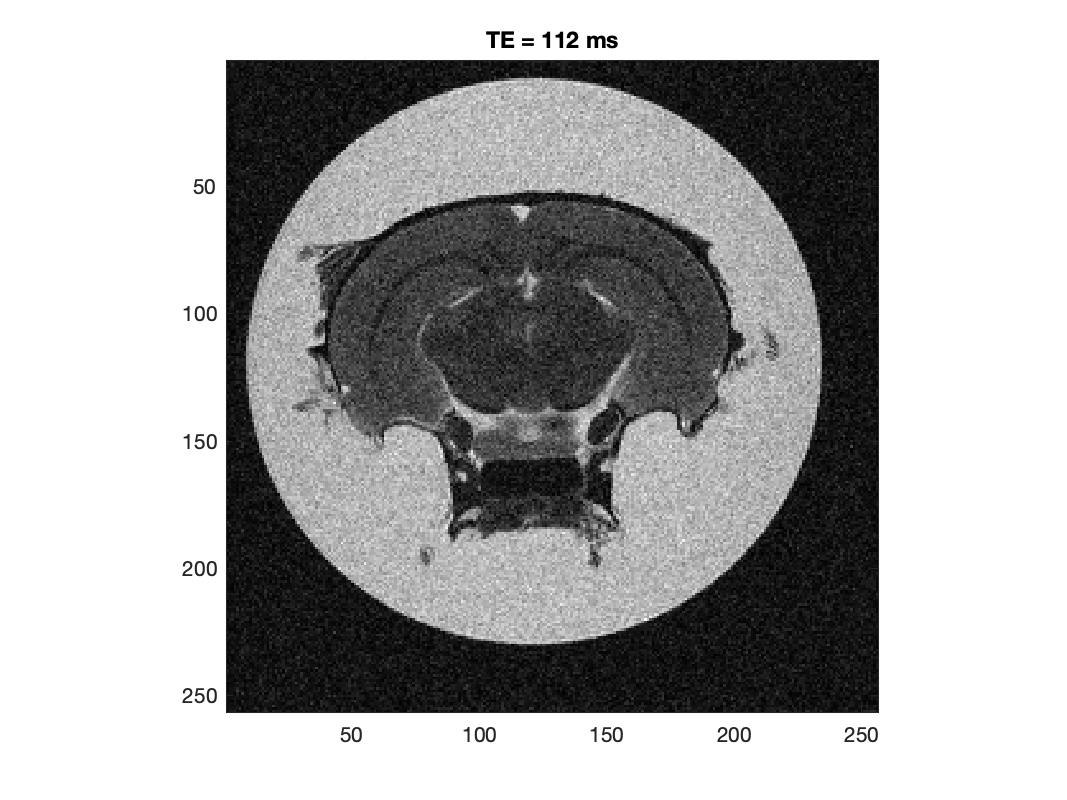
\includegraphics[width=0.15 \linewidth]{figures/MSME_6week/msme_6week_14.png}
						&
						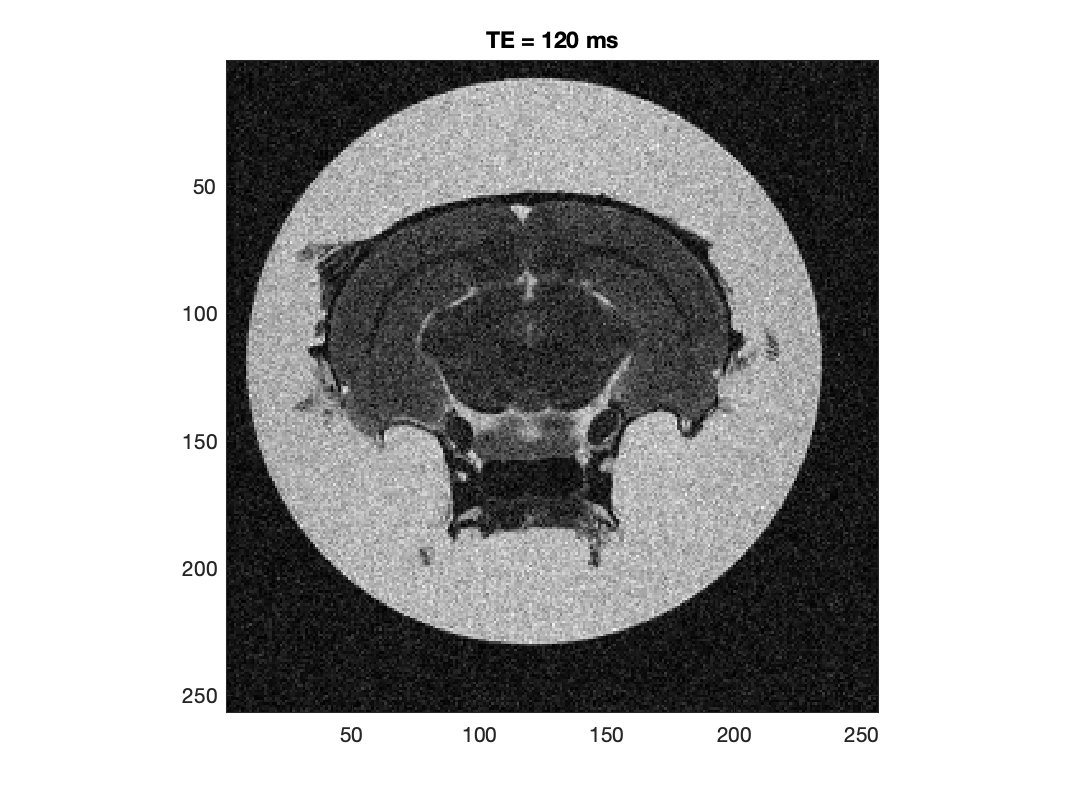
\includegraphics[width=0.15 \linewidth]{figures/MSME_6week/msme_6week_15.png}
						&
						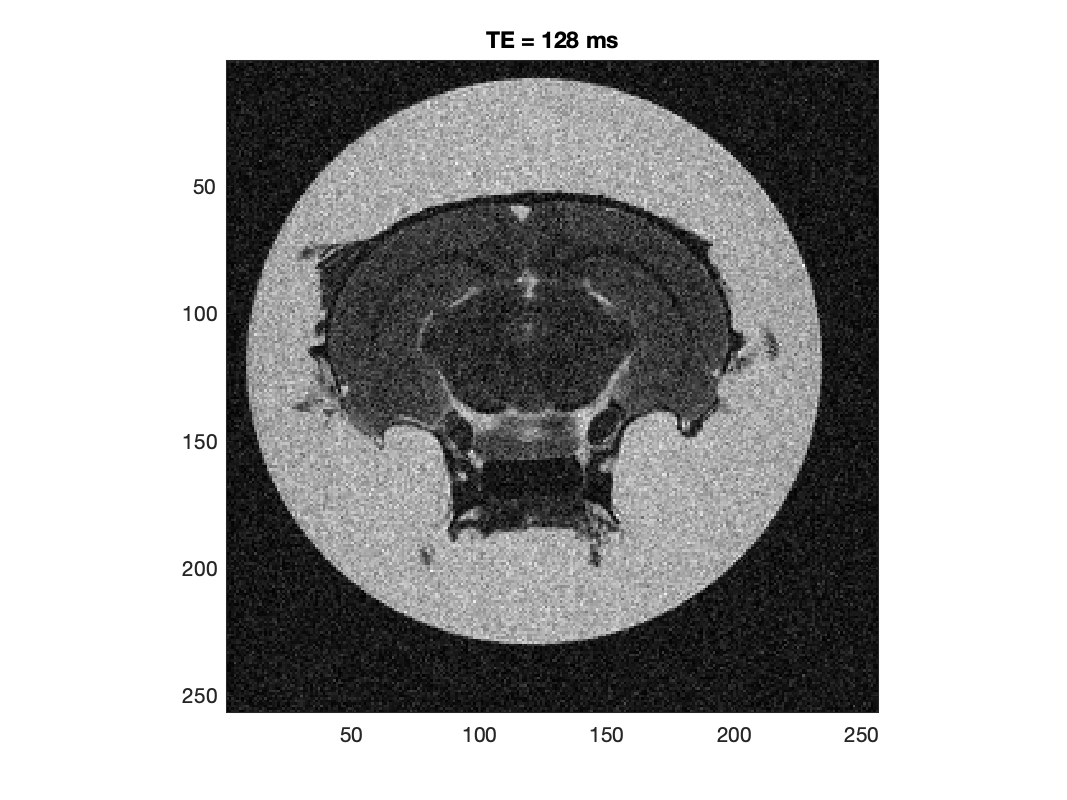
\includegraphics[width=0.15 \linewidth]{figures/MSME_6week/msme_6week_16.png}
						&
						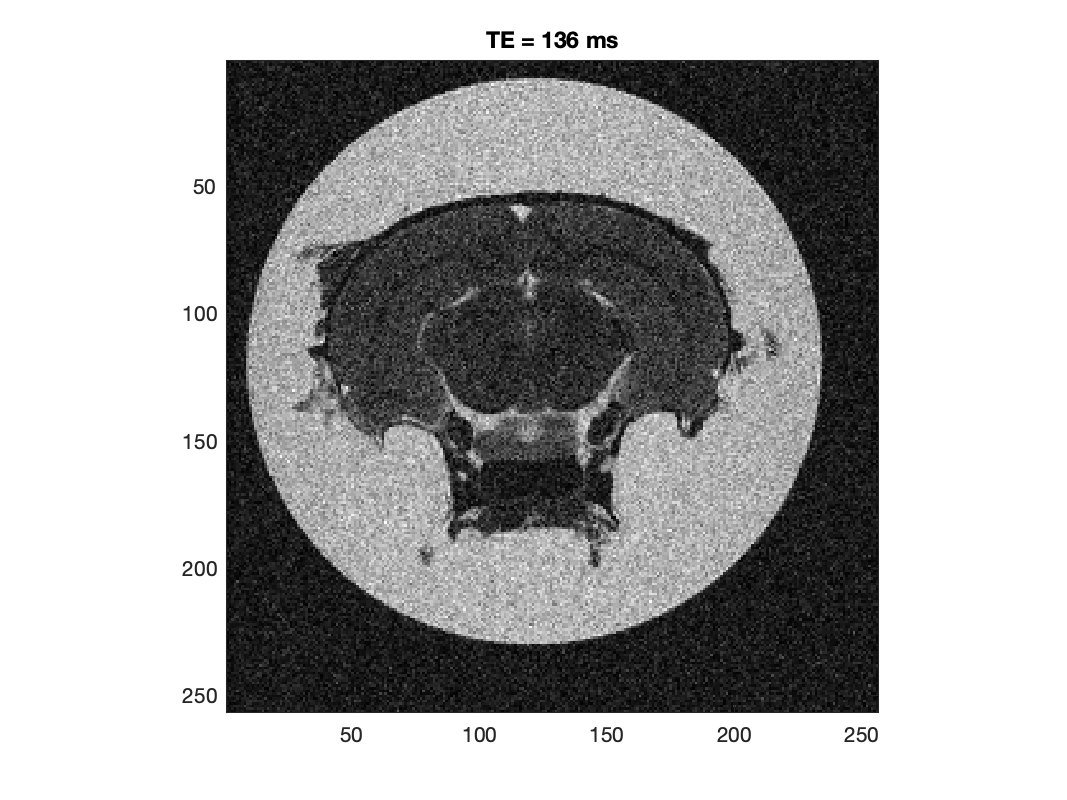
\includegraphics[width=0.15 \linewidth]{figures/MSME_6week/msme_6week_17.png}
						&
						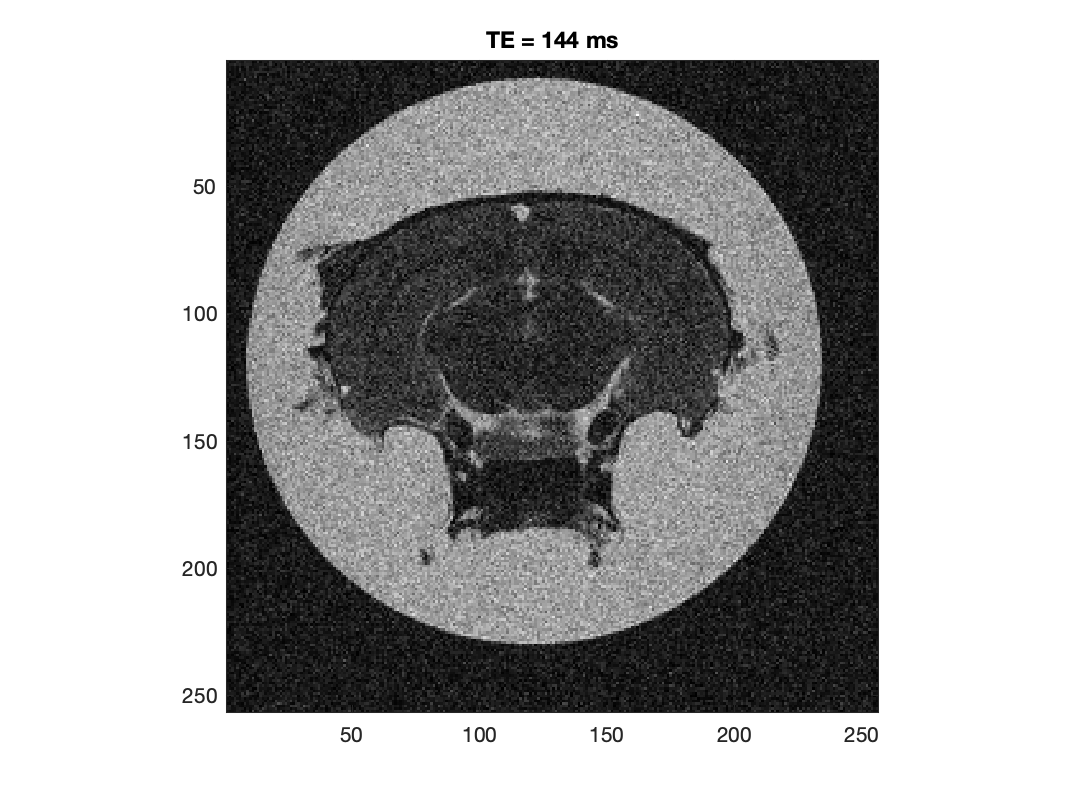
\includegraphics[width=0.15 \linewidth]{figures/MSME_6week/msme_6week_18.png}
						\\
						\mbox{(13)} & \mbox{(14)} & \mbox{(15)} & \mbox{(16)} & \mbox{(17)} & \mbox{(18)} \\
						
						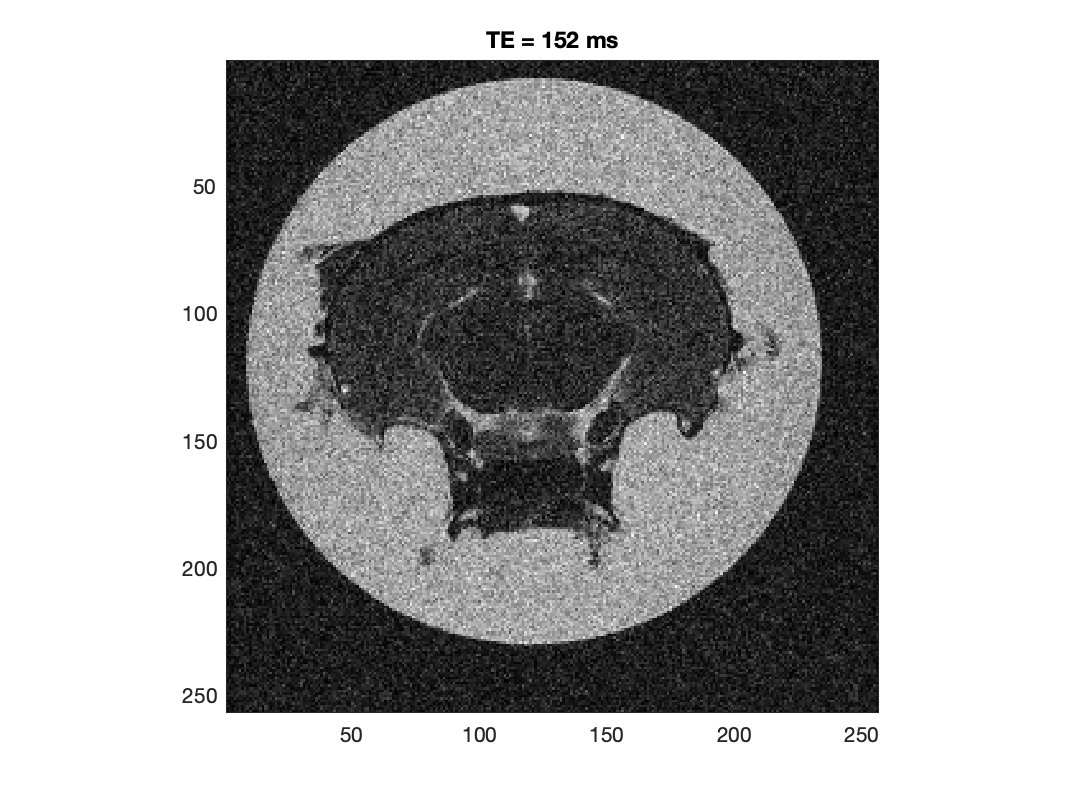
\includegraphics[width=0.15 \linewidth]{figures/MSME_6week/msme_6week_19.png}
						&
						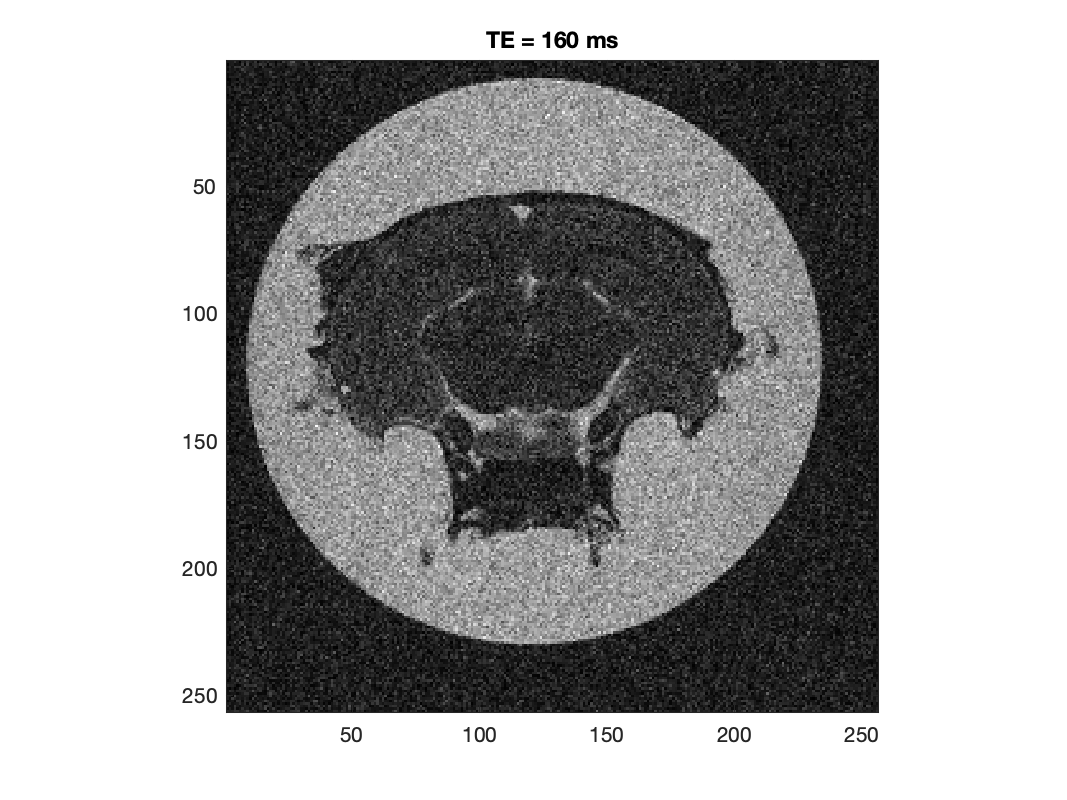
\includegraphics[width=0.15 \linewidth]{figures/MSME_6week/msme_6week_20.png}
						&
						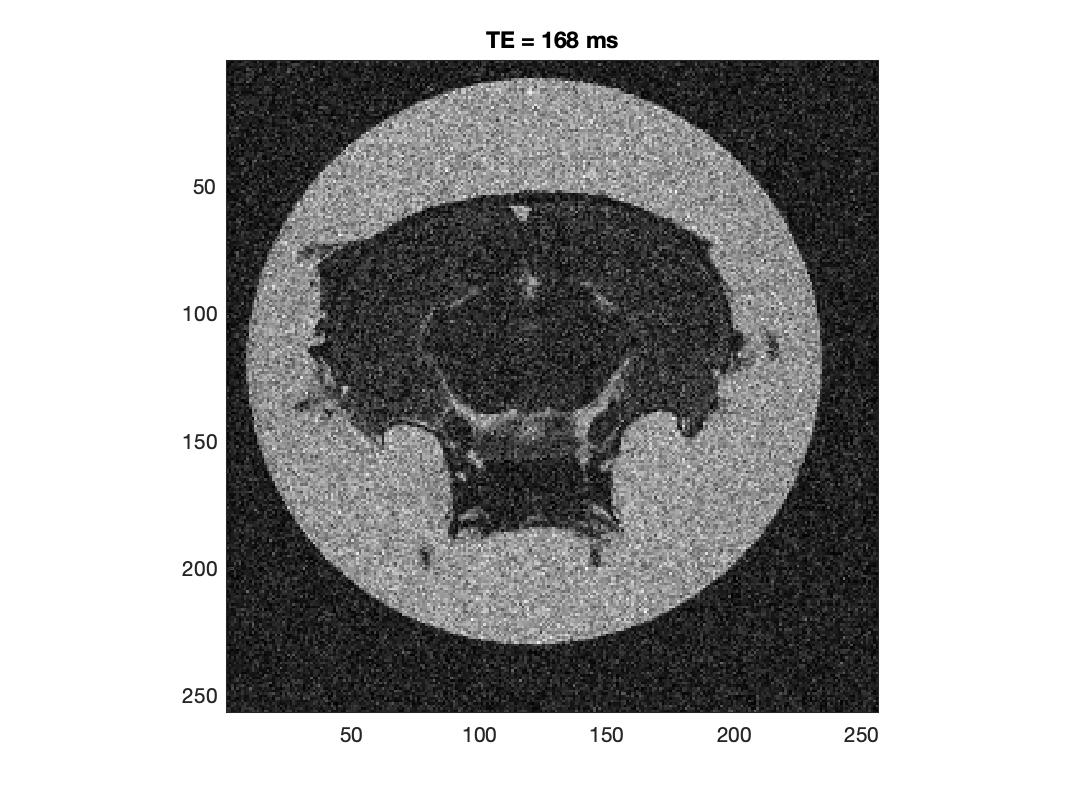
\includegraphics[width=0.15 \linewidth]{figures/MSME_6week/msme_6week_21.png}
						&
						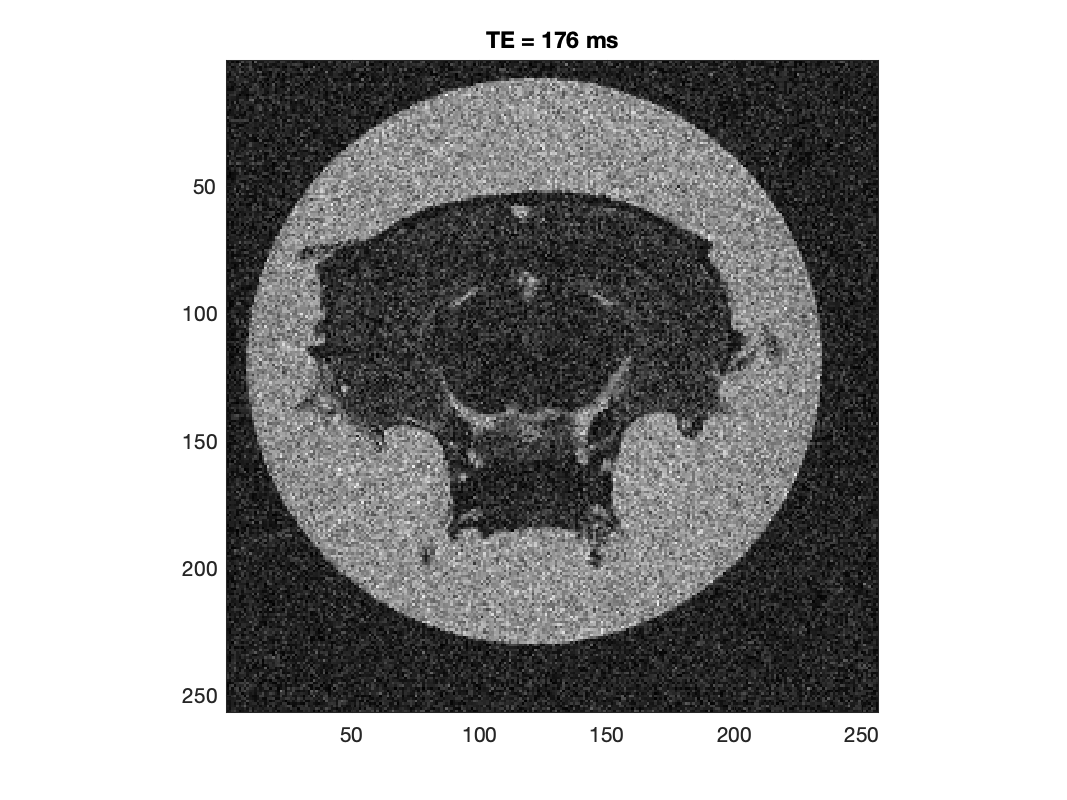
\includegraphics[width=0.15 \linewidth]{figures/MSME_6week/msme_6week_22.png}
						&
						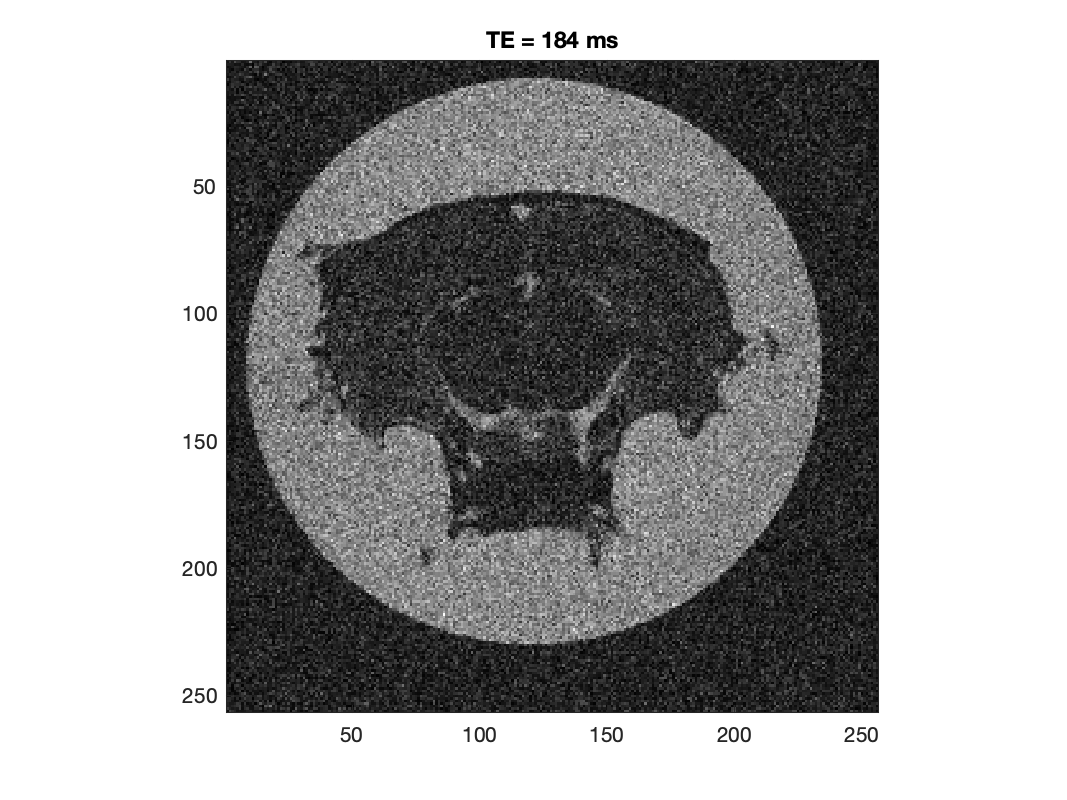
\includegraphics[width=0.15 \linewidth]{figures/MSME_6week/msme_6week_23.png}
						&
						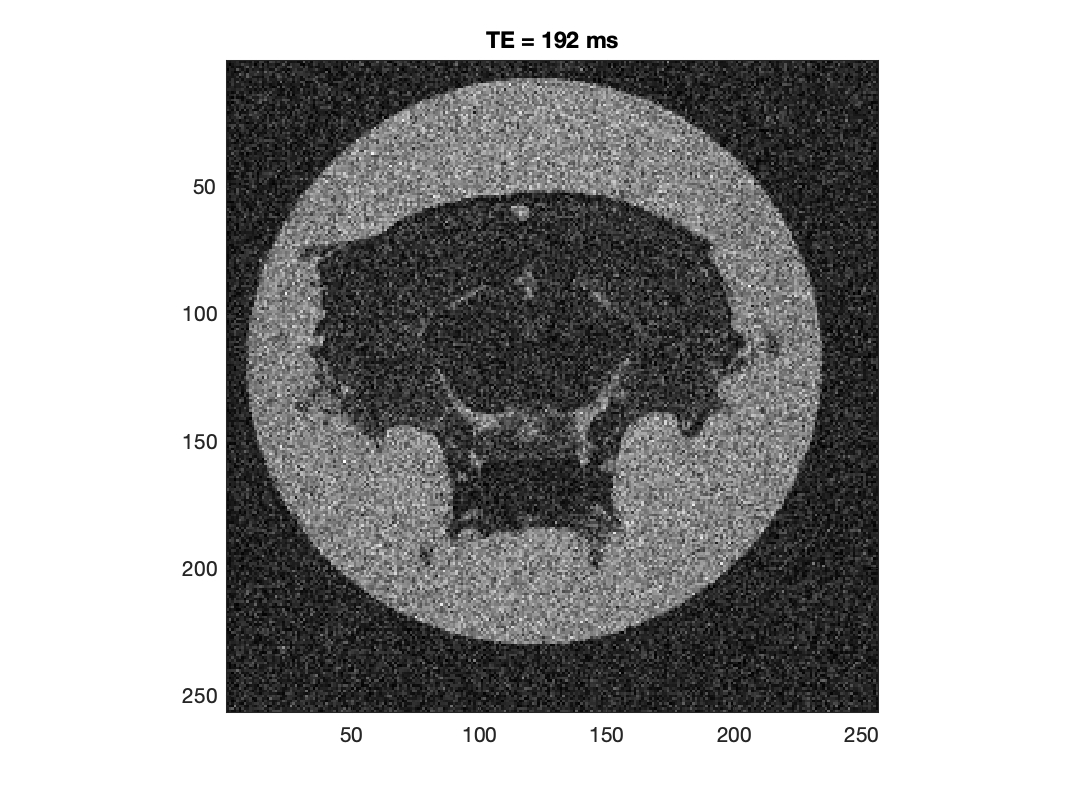
\includegraphics[width=0.15 \linewidth]{figures/MSME_6week/msme_6week_24.png}
						\\
						\mbox{(19)} & \mbox{(20)} & \mbox{(21)} & \mbox{(22)} & \mbox{(23)} & \mbox{(24)} \\
						
						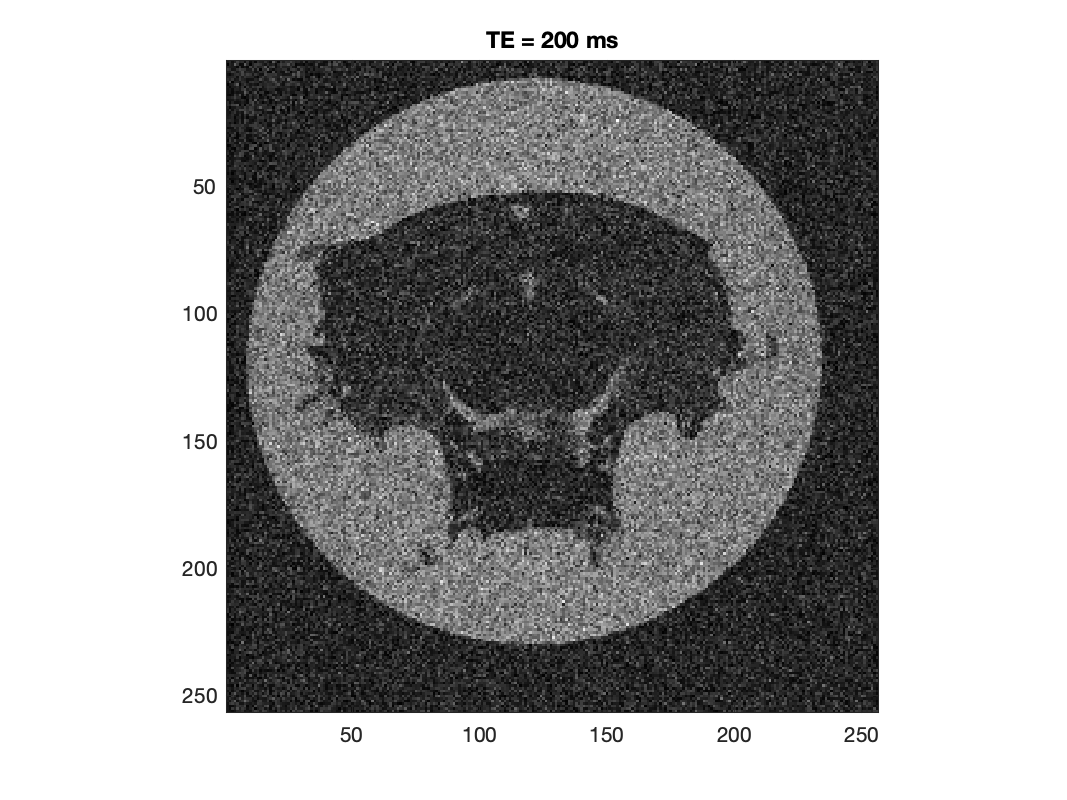
\includegraphics[width=0.15 \linewidth]{figures/MSME_6week/msme_6week_25.png}
						&
						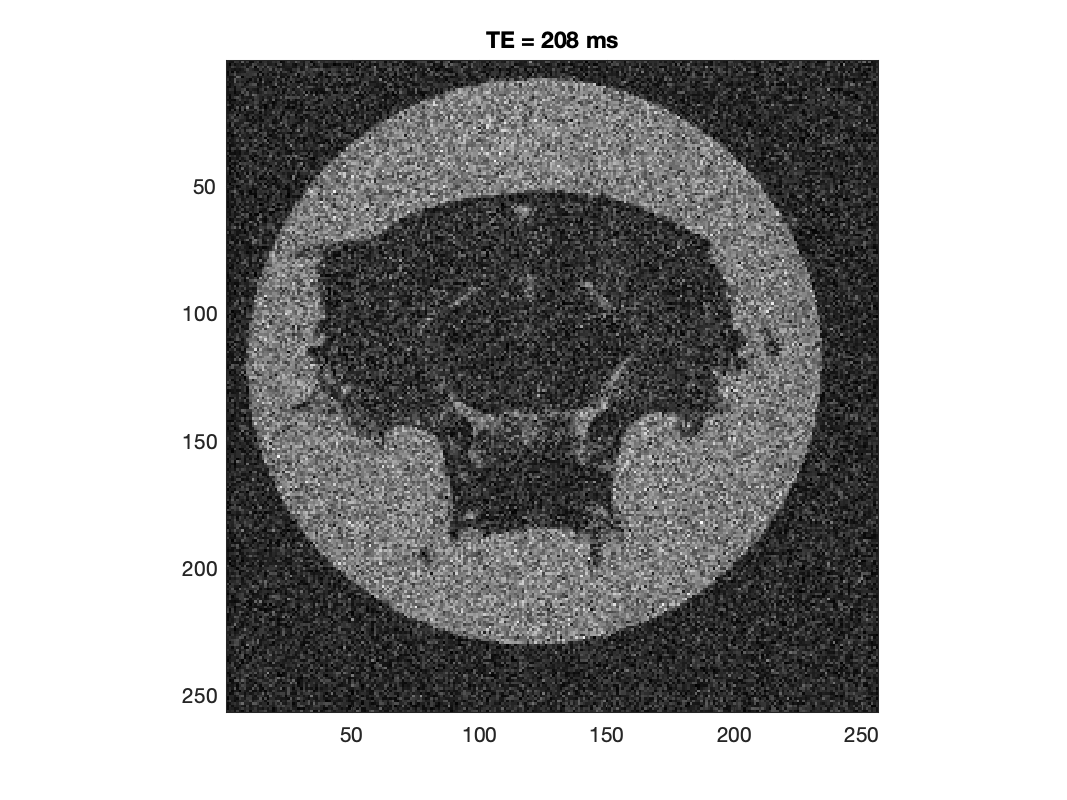
\includegraphics[width=0.15 \linewidth]{figures/MSME_6week/msme_6week_26.png}
						&
						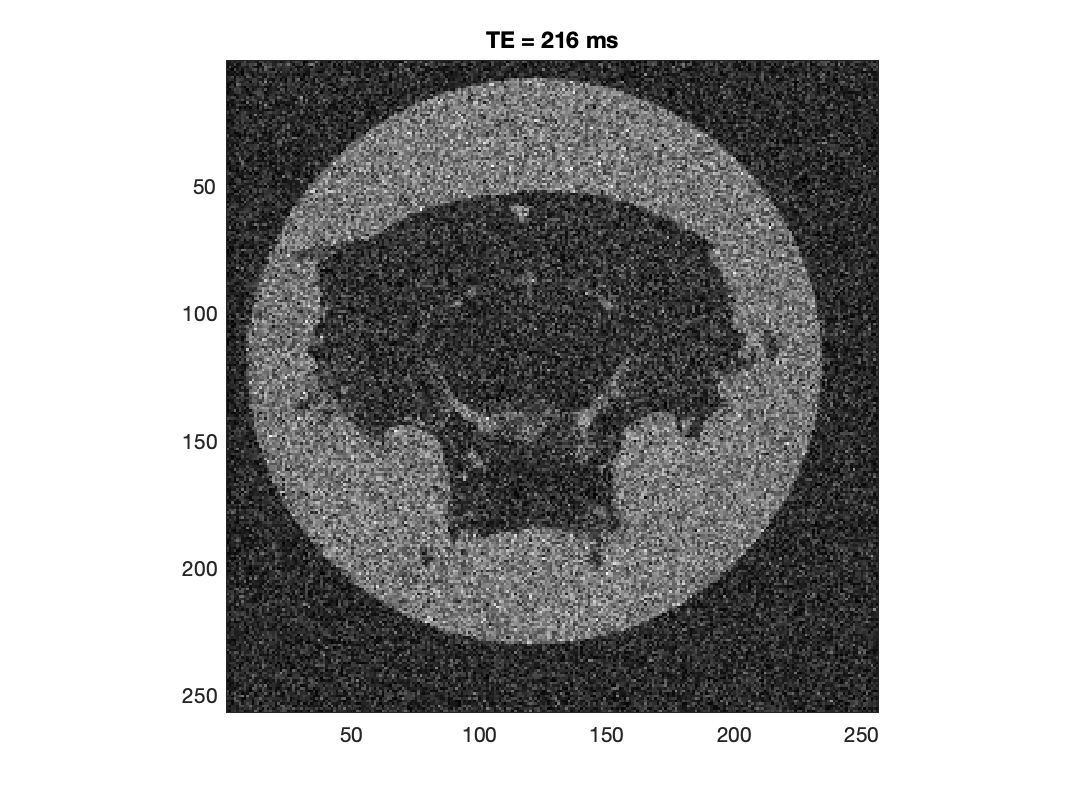
\includegraphics[width=0.15 \linewidth]{figures/MSME_6week/msme_6week_27.png}
						&
						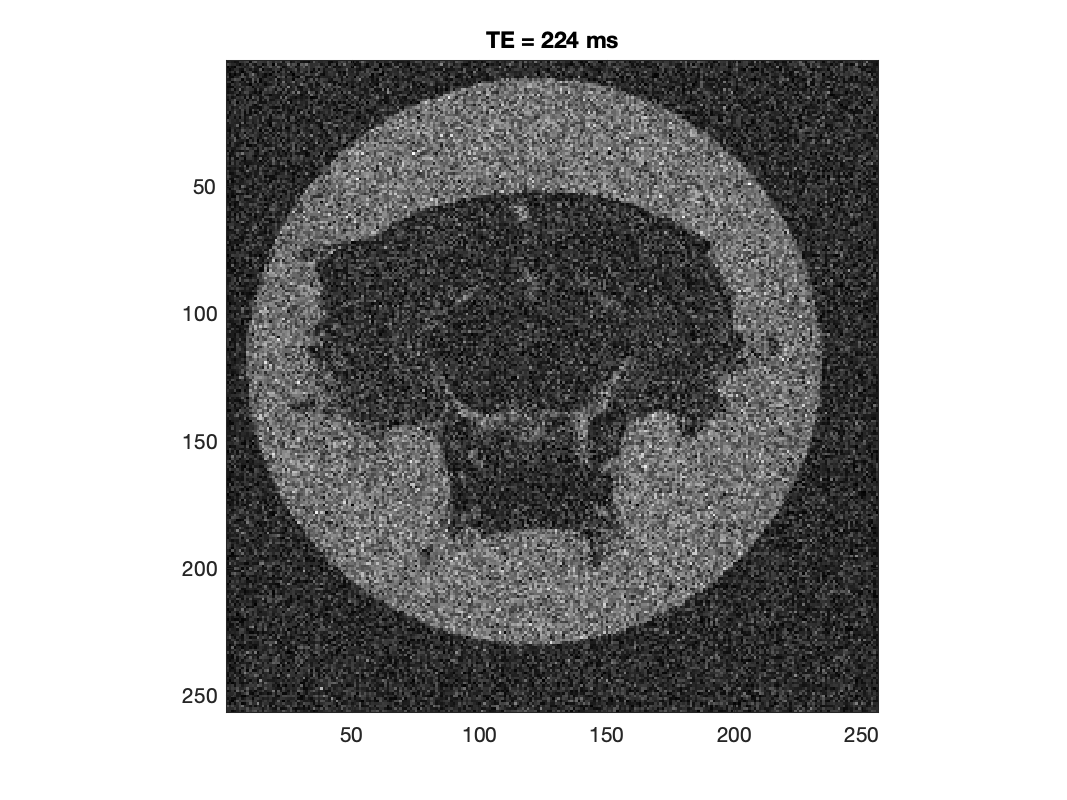
\includegraphics[width=0.15 \linewidth]{figures/MSME_6week/msme_6week_28.png}
						&
						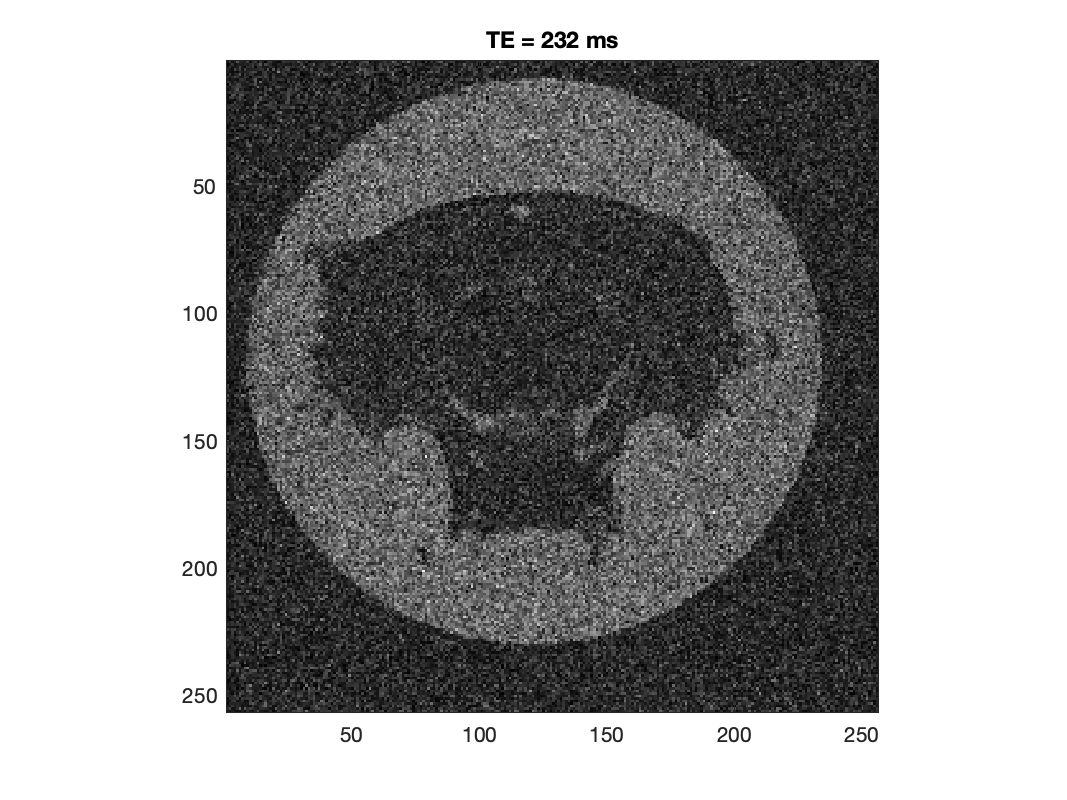
\includegraphics[width=0.15 \linewidth]{figures/MSME_6week/msme_6week_29.png}
						&
						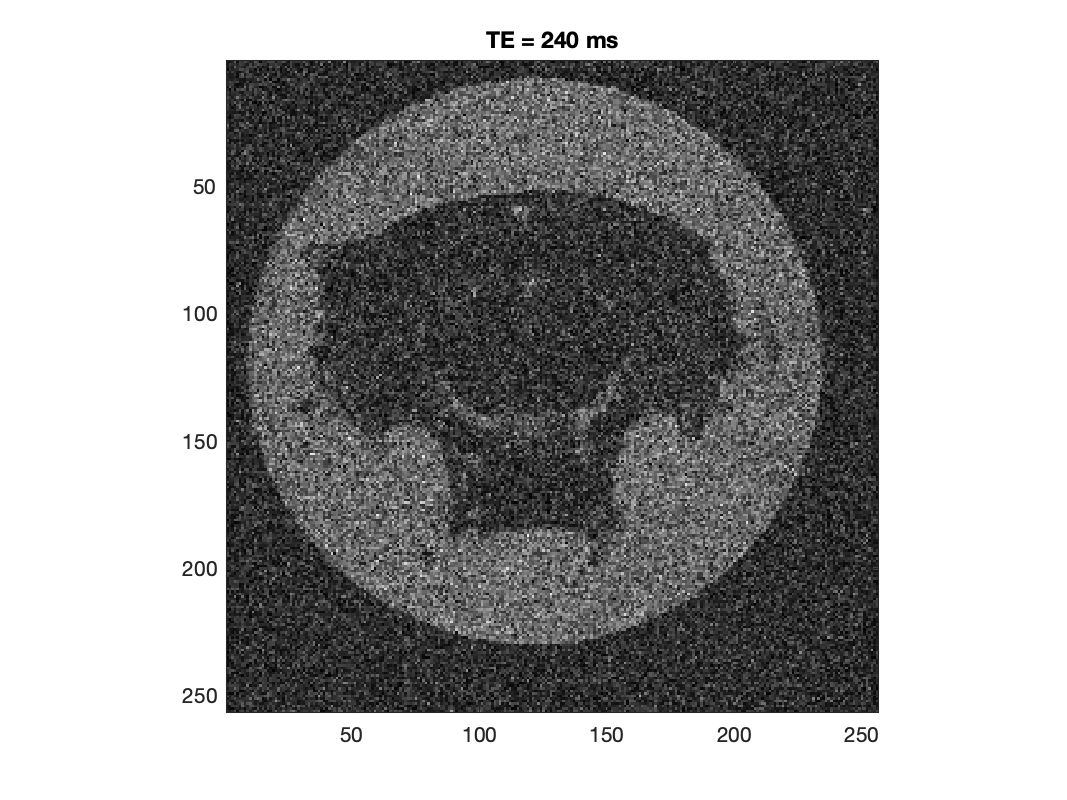
\includegraphics[width=0.15 \linewidth]{figures/MSME_6week/msme_6week_30.png}
						\\
						\mbox{(25)} & \mbox{(26)} & \mbox{(27)} & \mbox{(28)} & \mbox{(29)} & \mbox{(30)} \\
						
						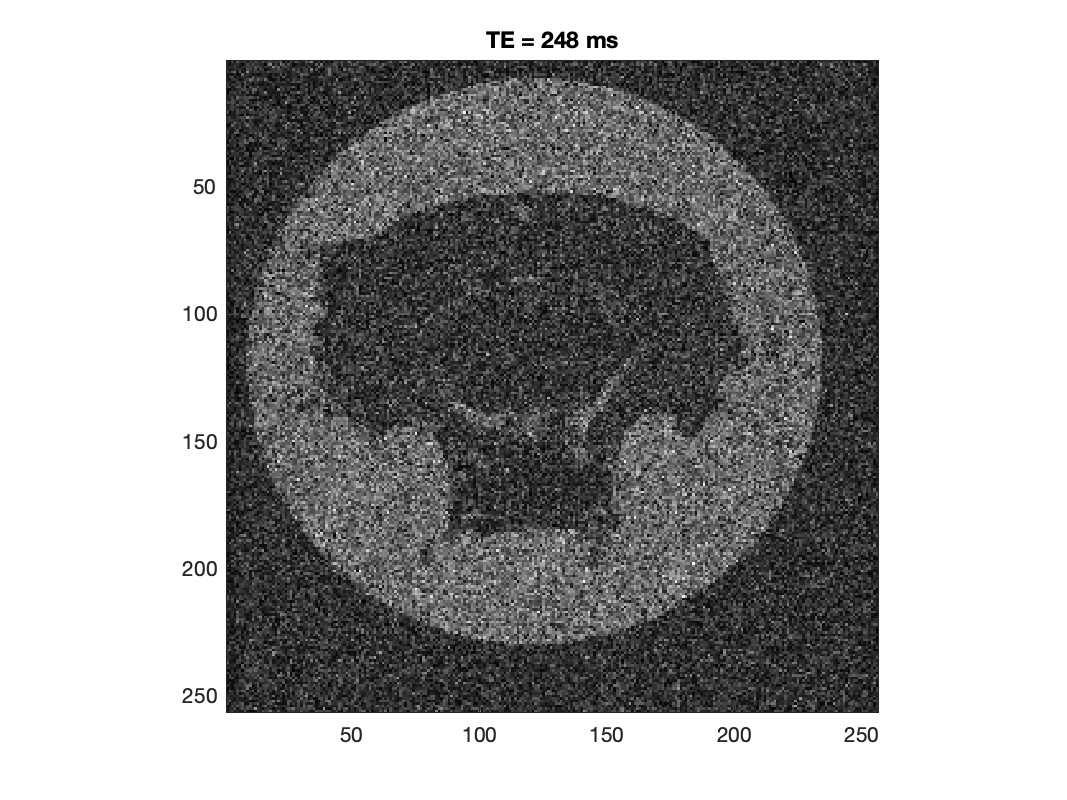
\includegraphics[width=0.15 \linewidth]{figures/MSME_6week/msme_6week_31.png}
						&
						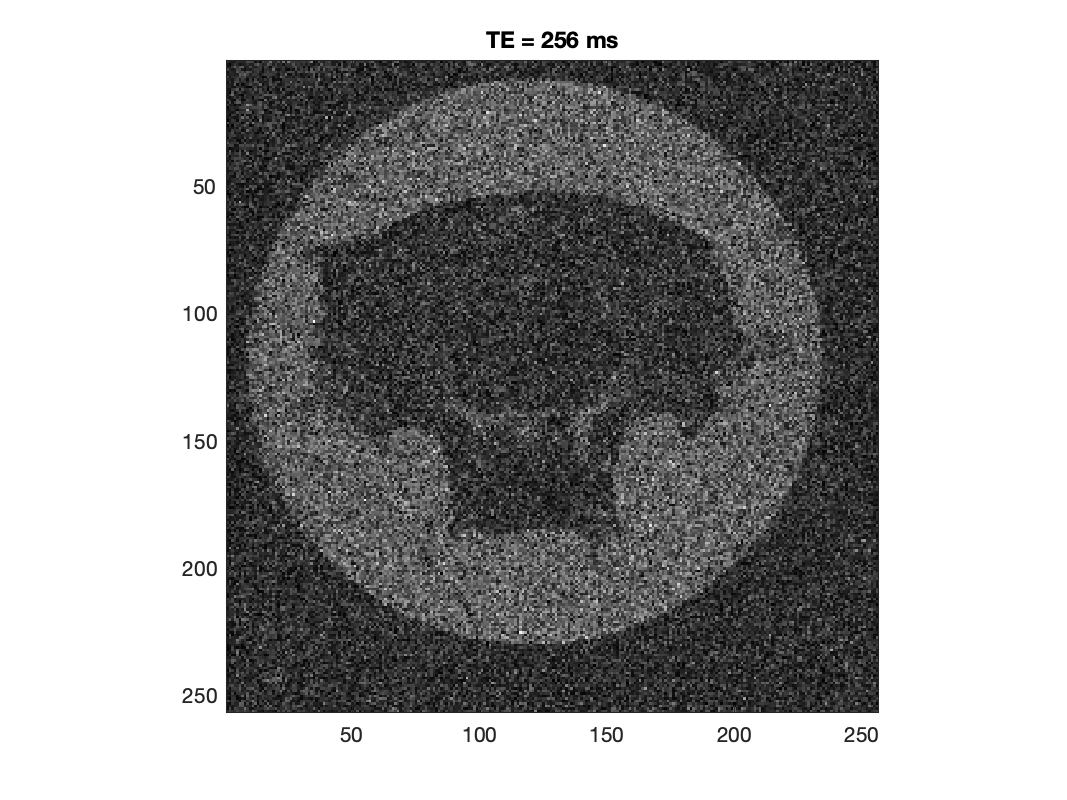
\includegraphics[width=0.15 \linewidth]{figures/MSME_6week/msme_6week_32.png}
						&
						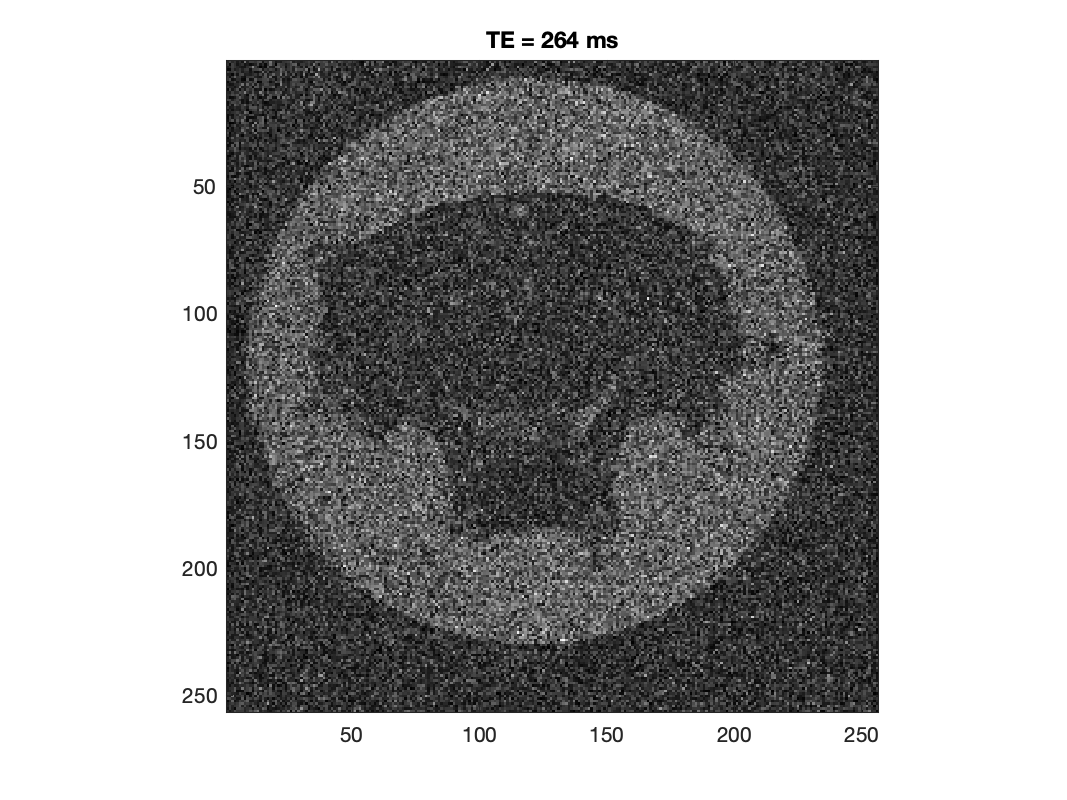
\includegraphics[width=0.15 \linewidth]{figures/MSME_6week/msme_6week_33.png}
						&
						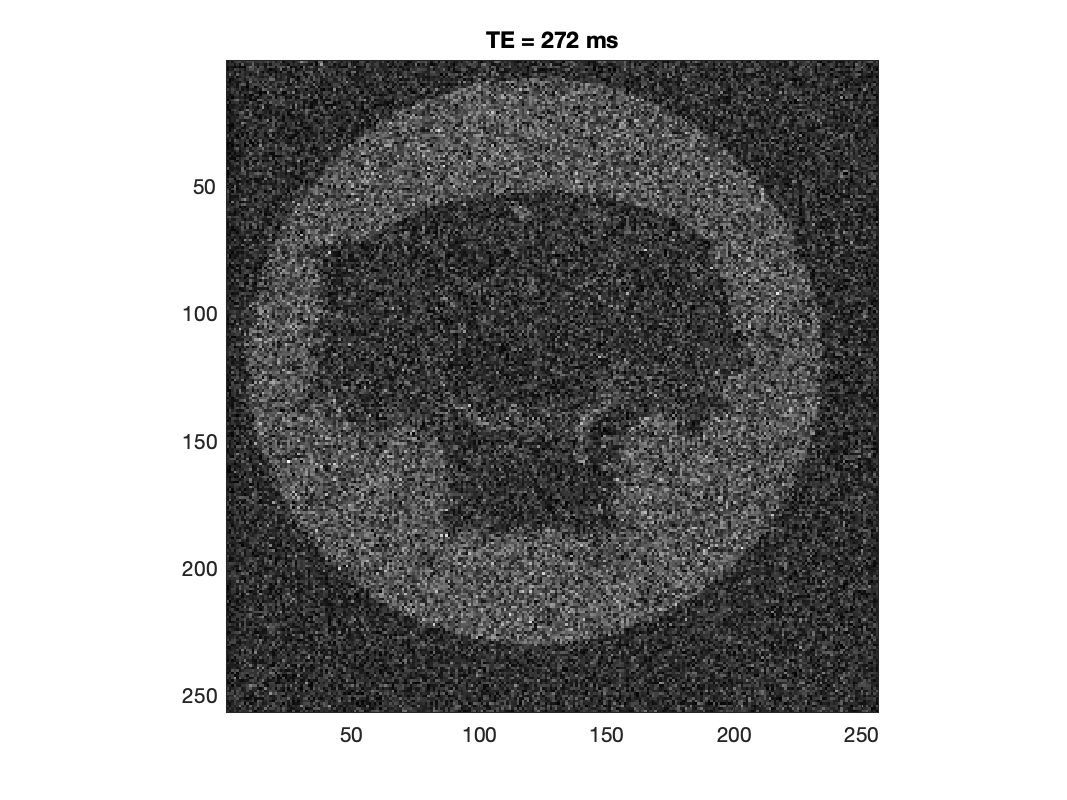
\includegraphics[width=0.15 \linewidth]{figures/MSME_6week/msme_6week_34.png}
						&
						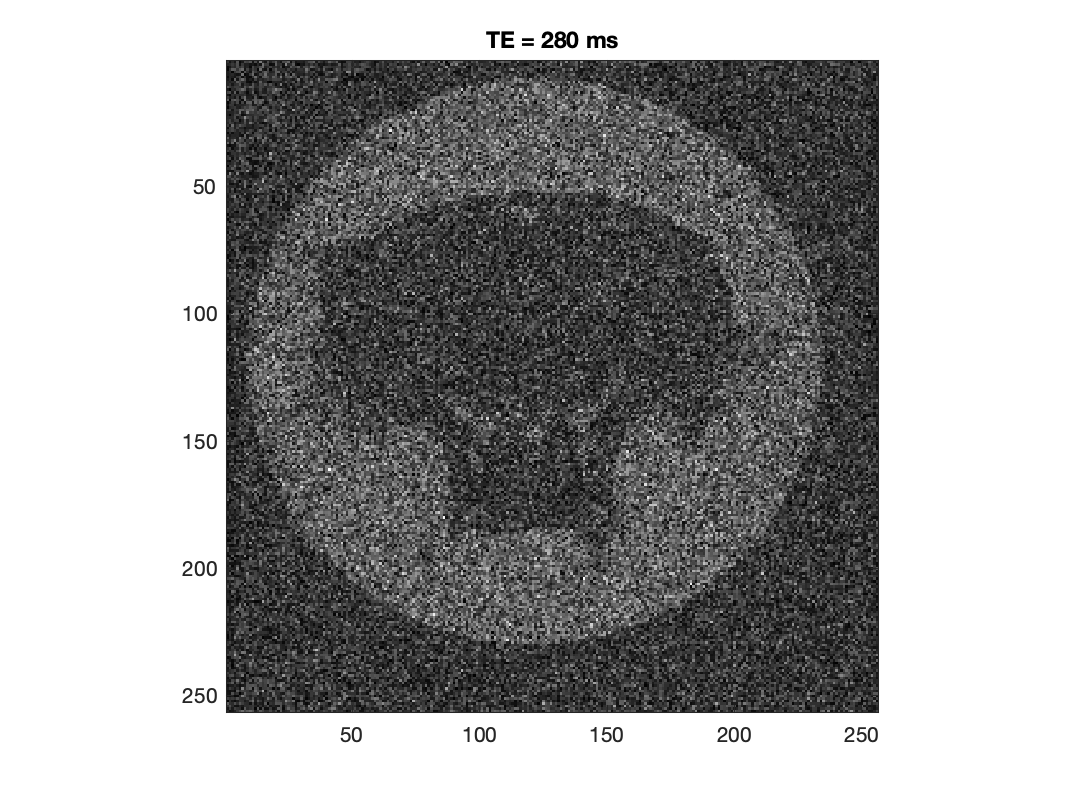
\includegraphics[width=0.15 \linewidth]{figures/MSME_6week/msme_6week_35.png}
						&
						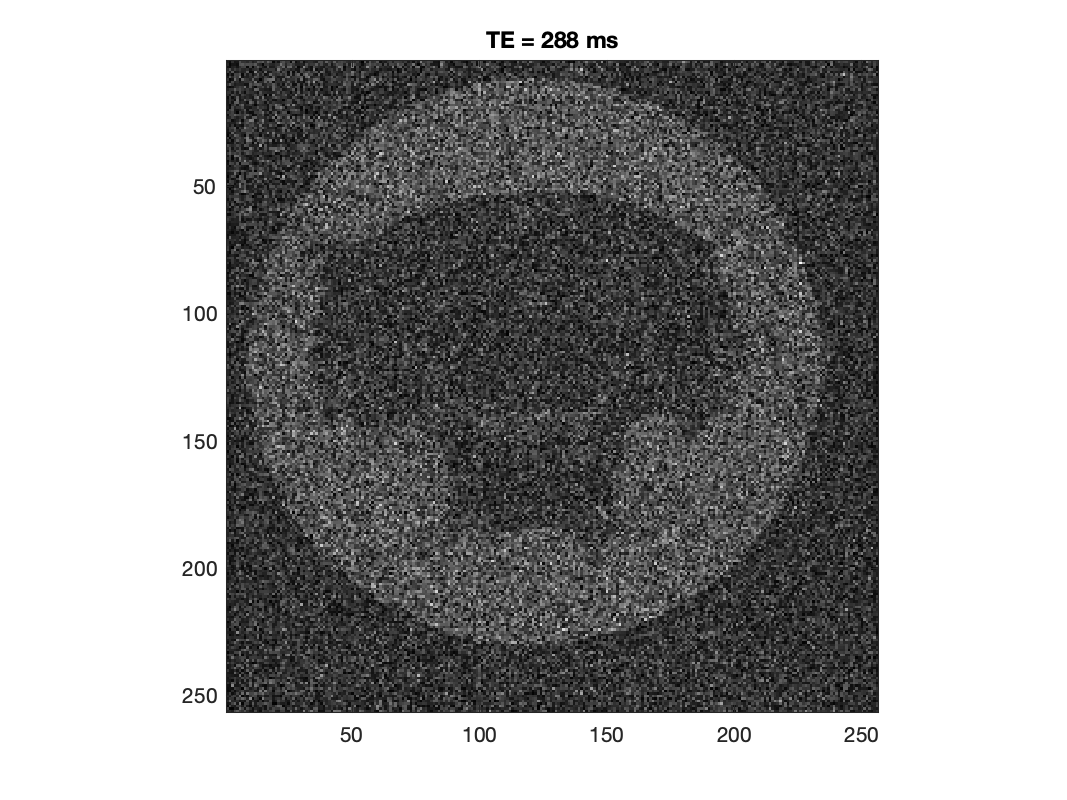
\includegraphics[width=0.15 \linewidth]{figures/MSME_6week/msme_6week_36.png}
						\\
						\mbox{(31)} & \mbox{(32)} & \mbox{(33)} & \mbox{(34)} & \mbox{(35)} & \mbox{(36)} \\
						
						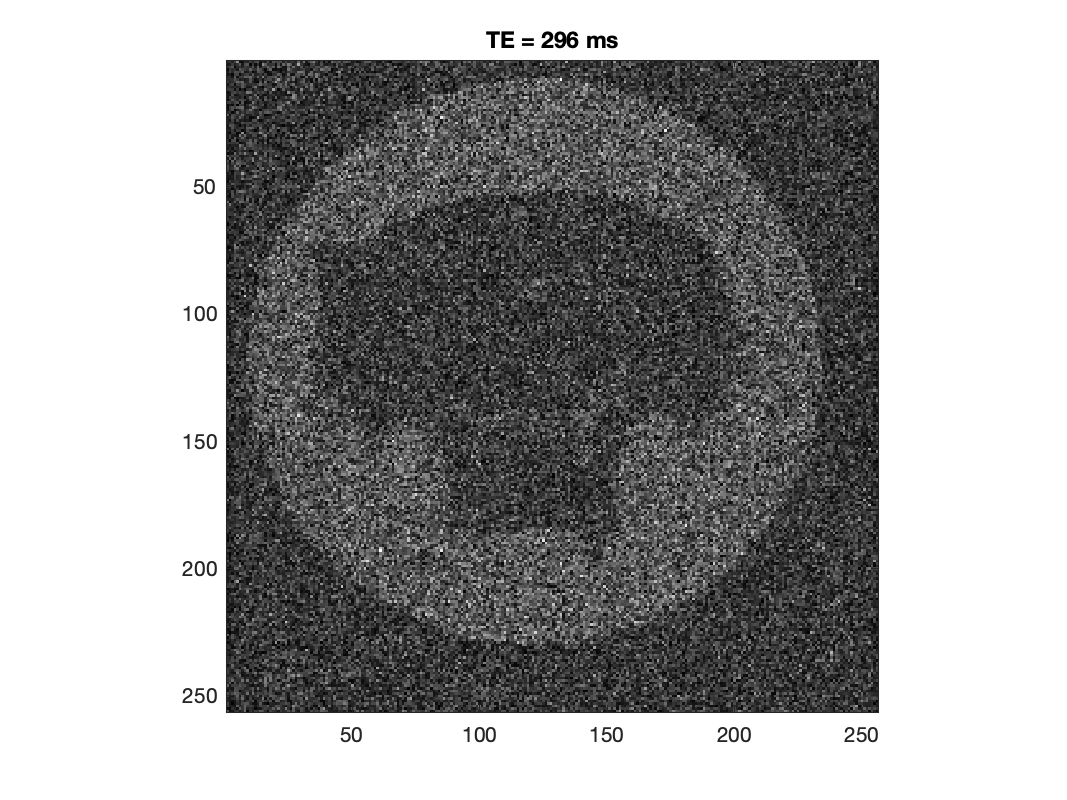
\includegraphics[width=0.15 \linewidth]{figures/MSME_6week/msme_6week_37.png}
						&
						\includegraphics[width=0.15 \linewidth]{figures/MSME_6week/msme_6week_38.png}
						&
						\includegraphics[width=0.15 \linewidth]{figures/MSME_6week/msme_6week_39.png}
						&
						\includegraphics[width=0.15 \linewidth]{figures/MSME_6week/msme_6week_40.png}
						&
						\includegraphics[width=0.15 \linewidth]{figures/MSME_6week/msme_6week_41.png}
						&
						\includegraphics[width=0.15 \linewidth]{figures/MSME_6week/msme_6week_42.png}
						\\
						\mbox{(37)} & \mbox{(38)} & \mbox{(39)} & \mbox{(40)} & \mbox{(41)} & \mbox{(42)} \\
						
						\includegraphics[width=0.15 \linewidth]{figures/MSME_6week/msme_6week_43.png}
						&
						\includegraphics[width=0.15 \linewidth]{figures/MSME_6week/msme_6week_44.png}
						&
						\includegraphics[width=0.15 \linewidth]{figures/MSME_6week/msme_6week_45.png}
						&
						\includegraphics[width=0.15 \linewidth]{figures/MSME_6week/msme_6week_46.png}
						&
						\includegraphics[width=0.15 \linewidth]{figures/MSME_6week/msme_6week_47.png}
						&
						\includegraphics[width=0.15 \linewidth]{figures/MSME_6week/msme_6week_48.png}
						\\
						\mbox{(43)} & \mbox{(44)} & \mbox{(45)} & \mbox{(46)} & \mbox{(47)} & \mbox{(48)} \\
					\end{array}$
					\caption{MSME FID Images in 6 Week}
					\label{fig:msme_6week_image}
				\end{figure}
			
			\subsubsection{MGE FID Image}
				In the figure \ref{fig:mge_6week_image}, there are 15 MRI images from MGE data. The TE is increasing on the figure \ref{fig:mge_6week_image}. By comparing the image \ref{fig:mge_6week_image}-(1) and the image \ref{fig:mge_6week_image}-(15), decreasing TR is enhancing the $T_2^*$ weighted image. 
				\begin{figure}[htbp]
					\centering
					$\begin{array}{ccc}
						\includegraphics[width=0.3 \linewidth]{figures/MGE_6week/mge_6week_1.png}
						&
						\includegraphics[width=0.3 \linewidth]{figures/MGE_6week/mge_6week_2.png}
						&
						\includegraphics[width=0.3 \linewidth]{figures/MGE_6week/mge_6week_3.png}
						\\
						\mbox{(1)} & \mbox{(2)} & \mbox{(3)} \\
						
						\includegraphics[width=0.3 \linewidth]{figures/MGE_6week/mge_6week_4.png}
						&
						\includegraphics[width=0.3 \linewidth]{figures/MGE_6week/mge_6week_5.png}
						&
						\includegraphics[width=0.3 \linewidth]{figures/MGE_6week/mge_6week_6.png}
						\\
						\mbox{(4)} & \mbox{(5)} & \mbox{(6)} \\
						
						\includegraphics[width=0.3 \linewidth]{figures/MGE_6week/mge_6week_7.png}
						&
						\includegraphics[width=0.3 \linewidth]{figures/MGE_6week/mge_6week_8.png}
						&
						\includegraphics[width=0.3 \linewidth]{figures/MGE_6week/mge_6week_9.png}
						\\
						\mbox{(7)} & \mbox{(8)} & \mbox{(9)} \\
						
						\includegraphics[width=0.3 \linewidth]{figures/MGE_6week/mge_6week_10.png}
						&
						\includegraphics[width=0.3 \linewidth]{figures/MGE_6week/mge_6week_11.png}
						&
						\includegraphics[width=0.3 \linewidth]{figures/MGE_6week/mge_6week_12.png}
						\\
						\mbox{(10} & \mbox{(11)} & \mbox{(12)} \\
						
						\includegraphics[width=0.3 \linewidth]{figures/MGE_6week/mge_6week_13.png}
						&
						\includegraphics[width=0.3 \linewidth]{figures/MGE_6week/mge_6week_14.png}
						&
						\includegraphics[width=0.3 \linewidth]{figures/MGE_6week/mge_6week_15.png}
						\\
						\mbox{(13)} & \mbox{(14)} & \mbox{(15)} \\
					\end{array}$
			
					\caption{MGE FID Images in 6 Week}
					\label{fig:mge_6week_image}
				\end{figure}
		
		\subsection{$T_1$, $T_2$, $T_2^*$ Fitting}
			In this section, $T_1$, $T_2$, and $T_2^*$ fitting will be performed. However, it is impossible that displaying all of the fitness in the one figure. In other word, the representative value should be selected, and the fitness on the representative value should be shown. Thus, the average value of signal stands for the representative value. 
			
			\subsubsection{$T_1$ Fitting}
				The $T_1$ fitting is displayed in the figure \ref{fig:t1_fitting}.
				\begin{figure}[htbp]
					\centering
					$\begin{array}{ccc}
						\includegraphics[width=0.3 \linewidth]{figures/T1_fit/T1_6week_fit.png}
						&
						\includegraphics[width=0.3 \linewidth]{figures/T1_fit/T1_4month_fit.png}
						&
						\includegraphics[width=0.3 \linewidth]{figures/T1_fit/T1_20month_fit.png}
						\\
						\mbox{(a) 6 Week} & \mbox{(b) 4 Month} & \mbox{(c) 20 Month} \\
					\end{array}$
					\caption{$T_1$ Fitting}
					\label{fig:t1_fitting}
				\end{figure}
			
			\subsubsection{$T_2$ Fitting}
				The $T_2$ fitting is displayed in the figure \ref{fig:t2_fitting}.
				\begin{figure}[htbp]
					\centering
					$\begin{array}{ccc}
					\includegraphics[width=0.3 \linewidth]{figures/T2_fit/T2_6week_fit.png}
					&
					\includegraphics[width=0.3 \linewidth]{figures/T2_fit/T2_4month_fit.png}
					&
					\includegraphics[width=0.3 \linewidth]{figures/T2_fit/T2_20month_fit.png}
					\\
					\mbox{(a) 6 Week} & \mbox{(b) 4 Month} & \mbox{(c) 20 Month} \\
					\end{array}$
					\caption{$T_2$ Fitting}
					\label{fig:t2_fitting}
				\end{figure}
			
			\subsubsection{$T_2^*$ Fitting}
				The $T_2^*$ fitting is displayed in the figure \ref{fig:t2star_fitting}.
				\begin{figure}[htbp]
					\centering
					$\begin{array}{ccc}
					\includegraphics[width=0.3 \linewidth]{figures/T2star_fit/T2star_6week_fit.png}
					&
					\includegraphics[width=0.3 \linewidth]{figures/T2star_fit/T2star_4month_fit.png}
					&
					\includegraphics[width=0.3 \linewidth]{figures/T2star_fit/T2star_20month_fit.png}
					\\
					\mbox{(a) 6 Week} & \mbox{(b) 4 Month} & \mbox{(c) 20 Month} \\
					\end{array}$
					\caption{$T_2^*$ Fitting}
					\label{fig:t2star_fitting}
				\end{figure}
		
		\subsection{$T_1$, $T_2$, $T_2^*$ Mapping}
			In this section, $T_1$, $T_2$, and $T_2^*$ fitting is performed on every voxels. However, the $R^2$ values are ignored, because $R^2 > 0.95$ is satisfied upon every voxels.
		
			\subsubsection{$T_1$ Mapping}
				The $T_1$ mapping is shown as the figure \ref{fig:t1_mapping}. Note that, in some voxels on side, the $T_1$ is estimated as $T_1 > 10^7$. For handling this case, the maximum value is set as 2000. 
				\begin{figure}[htbp]
					\centering
					$\begin{array}{ccc}
						\includegraphics[width=0.3 \linewidth]{figures/T1_map/T1_6week_map.png}
						&
						\includegraphics[width=0.3 \linewidth]{figures/T1_map/T1_4month_map.png}
						&
						\includegraphics[width=0.3 \linewidth]{figures/T1_map/T1_20month_map.png}
						\\
						\mbox{(a) 6 Week} & \mbox{(b) 4 Month} & \mbox{(c) 20 Month} \\
					\end{array}$
					\caption{$T_1$ Mapping}
					\label{fig:t1_mapping}
				\end{figure}
			
			\subsubsection{$T_2$ Mapping}
				The $T_2$ mapping is shown as the figure \ref{fig:t2_mapping}. Note that, in some voxels on side, the $T_2$ is estimated as $T_2 > 10^7$. For handling this case, the maximum value is set as 50. 
				\begin{figure}[htbp]
					\centering
					$\begin{array}{ccc}
					\includegraphics[width=0.3 \linewidth]{figures/T2_map/T2_6week_map.png}
					&
					\includegraphics[width=0.3 \linewidth]{figures/T2_map/T2_4month_map.png}
					&
					\includegraphics[width=0.3 \linewidth]{figures/T2_map/T2_20month_map.png}
					\\
					\mbox{(a) 6 Week} & \mbox{(b) 4 Month} & \mbox{(c) 20 Month} \\
					\end{array}$
					\caption{$T_2$ Mapping}
					\label{fig:t2_mapping}
				\end{figure}
			
			\subsubsection{$T_2^*$ Mapping}
				The $T_2^*$ mapping is shown as the figure \ref{fig:t2star_mapping}. Note that, in some voxels on side, the $T_2^*$ is estimated as $T_2^* > 10^7$. For handling this case, the maximum value is set as 50. 
				\begin{figure}[htbp]
					\centering
					$\begin{array}{ccc}
					\includegraphics[width=0.3 \linewidth]{figures/T2star_map/T2star_6week_map.png}
					&
					\includegraphics[width=0.3 \linewidth]{figures/T2star_map/T2star_4month_map.png}
					&
					\includegraphics[width=0.3 \linewidth]{figures/T2star_map/T2star_20month_map.png}
					\\
					\mbox{(a) 6 Week} & \mbox{(b) 4 Month} & \mbox{(c) 20 Month} \\
					\end{array}$
					\caption{$T_2$ Mapping}
					\label{fig:t2star_mapping}
				\end{figure}
	
	\section{Discussion}
		\subsection{FID Data Reconstruction}
			As I mentioned herein-above, increasing TR is improving the image quality as the figure \ref{fig:vtr_6week_image}. Decreasing TE, however, is enhancing the image sharpness as the figures \ref{fig:msme_6week_image} and \ref{fig:mge_6week_image}.
			
		\subsection{$T_1$, $T_2$, $T_2^*$ Fitting}
			The fitted $T_1$, $T_2$, and $T_2^*$ values are in the figures \ref{fig:t1_fitting}, \ref{fig:t2_fitting}, and \ref{fig:t2star_fitting}. In every cases, $R^2 > 0.95$ is satisfied; In other words, the FID data with high confidence had been acquired. 
		
		\subsection{$T_1$, $T_2$, $T_2^*$ Mapping}
			The mapped $T_1$, $T_2$, and $T_2^*$ values are in the figures \ref{fig:t1_mapping}, \ref{fig:t2_mapping}, and \ref{fig:t2star_mapping}. In most cases, the voxels in out of the brain tissue have huge values; it might be caused by fitting on the no signal. 
		
		\subsection{Analysis by Age}
			The figure \ref{fig:vtr_age} shows that the RARE-VTR FID images along development. In the figure \ref{fig:vtr_age}, the images are selected by the highest sharpness. 
			
			\begin{figure}[htbp]
				\centering
				$\begin{array}{ccc}
					\includegraphics[width=0.3 \linewidth]{figures/VTR_6week/vtr_6week_10.png}
					&
					\includegraphics[width=0.3 \linewidth]{figures/VTR_4month/vtr_4month_10.png}
					&
					\includegraphics[width=0.3 \linewidth]{figures/VTR_20month/vtr_20month_10.png}
					\\
					\mbox{(a) 6 Week} & \mbox{(b) 4 Month} & \mbox{(c) 20 Month} \\
				\end{array}$
				\caption{RARE-VTR FID Images by Age}
				\label{fig:vtr_age}
			\end{figure}
		
			The figure \ref{fig:msme_age} exposes that the MSME FID images along development. In the figure \ref{fig:msme_age}, the images are selected by the contrast between each tissues. 
			\begin{figure}[htbp]
				\centering
				$\begin{array}{ccc}
					\includegraphics[width=0.3 \linewidth]{figures/MSME_6week/msme_6week_10.png}
					&
					\includegraphics[width=0.3 \linewidth]{figures/MSME_4month/msme_4month_10.png}
					&
					\includegraphics[width=0.3 \linewidth]{figures/MSME_20month/msme_20month_10.png}
					\\
					\mbox{(a) 6 Week} & \mbox{(b) 4 Month} & \mbox{(c) 20 Month} \\
				\end{array}$
				\caption{MSME FID Images by Age}
				\label{fig:msme_age}
			\end{figure}
		
			The figure \ref{fig:mge_age} publishes that the MGE FID images along development. In the figure \ref{fig:mge_age}, the images are selected by the contrast between each tissues. 
			\begin{figure}[htbp]
				\centering
				$\begin{array}{ccc}
					\includegraphics[width=0.3 \linewidth]{figures/MGE_6week/mge_6week_3.png}
					&
					\includegraphics[width=0.3 \linewidth]{figures/MGE_4month/mge_4month_3.png}
					&
					\includegraphics[width=0.3 \linewidth]{figures/MGE_20month/mge_20month_3.png}
					\\
					\mbox{(a) 6 Week} & \mbox{(b) 4 Month} & \mbox{(c) 20 Month} \\
				\end{array}$
				\caption{MGE FID Images by Age}
				\label{fig:mge_age}
			\end{figure}
		
			\subsubsection{SN}
				Comparing the SN in the image \ref{fig:vtr_age}-(a) versus the image \ref{fig:vtr_age}-(b) versus the image \ref{fig:vtr_age}-(c); there are dark part has been appeared between (a) and (b); however, the dark part will be disappear between (b) and (c). The figure \ref{fig:vtr_age} is RARE-VTR FID image; id est, the figure \ref{fig:vtr_age} is $T_1$ weighted image. Thus, cerebrospinal fluid (CSF) appears black on $T_1$ weighted image. 
				
				Furthermore, the dark part has showed in the figures \ref{fig:msme_age} and \ref{fig:mge_age}. As I mentioned above, MSME FID image and MGE FID image are $T_2$ and $T_2^*$ weighted images, respectively. Thus, fat and CSF appear black on $T_2$ and $T_2^*$ weighted images.
				
				Therefore, the dark part in the SN is not fat nor CSF. It is believed that the dark part is empty area; is an intermediate part for pruning between neuron synapses. As referring the table \ref{tb:dev}, 4 month in rats is equivalent to 12 years in human; in other words, the rat is on adolescence. Many papers suggest that neural pruning or circuitry are performed in adolescence. \cite{ref:adol1, ref:adol2, ref:adol3} Thus, this is a typical result. 
				
				Moreover, as I mentioned herein-above, the SN has a major role in dopamine distribution. \cite{ref:nigra2, ref:nigra4} In other hands, there are many evidences which sustain the activity of dopamine system in adolescence. \cite{ref:dopa1, ref:dopa2, ref:dopa3} Hence, the SN plays a major roles in not only dopamine distribution, but also the development in adolescence. 
			
			\subsubsection{CC}
				By the figure \ref{fig:vtr_age}, the CC has been darker along the aging. The CC is also being darker in the figures \ref{fig:msme_age} and \ref{fig:mge_age}. As I mentioned in previous section, the dark area in all of the figures \ref{fig:vtr_age}, \ref{fig:msme_age}, and \ref{fig:mge_age} means empty area in the brain. 
				
				Thus, it means that the CC is making more sophisticated neuron synapses. Many research suggest that the size or shape of the CC have been changed by many factors, such as sex or aging. \cite{ref:sex1, ref:age1} Also, there are many evidences direct that the CC is exponentially grown in adolescence. \cite{ref:grow1, ref:grow2} Hence, the evidences sustained this result. 
	
	\bibliographystyle{apacite}
	\bibliography{reference}
\end{document}